\documentclass[final,12pt]{colt2018}

\title[The Externalities of Exploration and How Data Diversity Helps Exploitation]{The Externalities of Exploration and \\ How Data Diversity Helps Exploitation\titletag{\thanks{Extended abstract. Full version appears as \href{https://arxiv.org/abs/1806.00543}{CoRR arXiv:1806.00543 v\#1.}}}}

\usepackage{times}

\coltauthor{\Name{Manish Raghavan}\thanks{MR is supported by an NSF Graduate Research Fellowship (DGE-1650441). Work done while at Microsoft Research.} \Email{manish@cs.cornell.edu}\\
     \addr Cornell University
 \AND
 \Name{Aleksandrs Slivkins} \Email{slivkins@microsoft.com}\\
 \addr Microsoft Research
 \AND
 \Name{Jennifer Wortman Vaughan} \Email{jenn@microsoft.com}\\
 \addr Microsoft Research
 \AND
 \Name{Zhiwei Steven Wu} \Email{zsw@umn.edu}\\
 \addr Microsoft Research
 }


%%% Alex's macro
\newcommand{\ie}{{i.e.,~\xspace}}
\newcommand{\eg}{{e.g.,~\xspace}}
\newcommand{\Eg}{{E.g.,~\xspace}}
\newcommand{\xhdr}[1]{\vspace{2mm} \noindent{\bf #1}}
\newcommand{\polylog}{\operatornamewithlimits{polylog}}
\newcommand{\LDOTS}{\, ,\ \ldots\ ,}     % smart "..."
\newcommand{\Cel}[1]{{\lceil {#1} \rceil}}
\newcommand{\Flr}[1]{{\lfloor {#1} \rfloor}}
\newcommand{\eps}{\varepsilon}

\newcommand{\mE}{\mathcal{E}}
\newcommand{\mH}{\mathcal{H}}
\newcommand{\mX}{\mathcal{X}}

% OneLiners itemized list
\newcommand{\initOneLiners}{%
 	\setlength{\itemsep}{0pt}
	\setlength{\parsep }{0pt}
  	\setlength{\topsep }{0pt}     	
%      \usecounter{myLISTctr}
}
\newenvironment{OneLiners}[1][\ensuremath{\bullet}]
    {\begin{list}
        {#1}
        {\initOneLiners}}
    {\end{list}}

\newenvironment{proofof}[1][]
	{\begin{proof}{\bf of #1}}
	{\end{proof}}

% More Alex's notation -- algorithms
\newcommand{\term}[1]{\ensuremath{\mathtt{#1}}\xspace}
\newcommand{\OPT}{\term{OPT}}
\newcommand{\ALG}{\term{ALG}}

\newcommand{\simF}{\term{sim}} % simulation function for D3.

% context tuples
\newcommand{\con}{\term{con}} % one context tuple
\newcommand{\CON}{\term{CON}} % set of all possible context tuples




\newcommand{\PReg}{\term{PReg}} % "prediction regret" in Greedy analysis
\newcommand{\rPReg}[1][{\rounds}]{\PReg^{#1}}  % restricted prediction regret
\newcommand{\rReg}[1][{\rounds}]{R^{#1}} % restricted regret

\newcommand{\PRegat}{\PReg^{\ALG}(\rounds)} % "prediction regret" in Greedy analysis

\newcommand{\bpreg}[1]{\PReg^{\rounds}(#1)}
\newcommand{\bpregi}[1]{\PReg^{#1}}
\newcommand{\bpregih}[2]{\PReg^{#1}(#2)}
\newcommand{\basereg}[1]{R_0^{\rounds}\left(#1\right)}
\newcommand{\baseregi}[1]{R_0^{#1}}
\newcommand{\reg}[1]{R(#1)}
\newcommand{\regi}[1]{R^{#1}}
\newcommand{\baseregih}[2]{R_0^{#1}(#2)}

\newcommand{\FRMR}{\term{FRmin\text{-}Reg}}
\newcommand{\MRMR}{\term{MRmin\text{-}Reg}}

\newcommand{\BayesGreedy}{BatchBayesGreedy\xspace}
\newcommand{\FreqGreedy}{BatchFreqGreedy\xspace}
\newcommand{\GreedyStyle}{batch-greedy-style\xspace}

\newcommand{\Rew}[1][\theta]{\mathtt{Rew}_{#1}} % reward function from Greedy analysis

\def\rounds{\mc T}


\usepackage{cleveref}
\usepackage{color}
\usepackage{tikz}
\newtheorem{fact}[theorem]{Fact}
\newtheorem{claim}[theorem]{Claim}
\def\R{\mathbb{R}}
\def\tran{^\top}

\newcommand{\p}[1]{\left(#1\right)}
\newcommand{\kl}[2]{\ensuremath{\text{KL}(#1 \, ||\, #2)}}
 \def\given{\;|\;}

\newcommand{\thetazero}{\theta^{(0)}}
\newcommand{\thetaone}{\theta^{(1)}}

\renewcommand{\b}[1]{\left[#1\right]}
\newcommand{\E}[1]{\mathbb{E}\b{#1}}
\newcommand{\D}{D}
\newcommand{\Dmin}{D_{\textrm{min}}}
\newcommand{\Dmaj}{D_{\textrm{maj}}}
\newcommand{\Mmin}{M_{\textrm{min}}}
\newcommand{\Mmaj}{M_{\textrm{maj}}}
%%% Manish's macros go here.
\newcommand\numberthis{\addtocounter{equation}{1}\tag{\theequation}}
\DeclareMathOperator*{\argmax}{arg\,max}
\DeclareMathOperator*{\argmin}{arg\,min}
\DeclareMathOperator{\Exp}{\mathbb{E}}
\def\R{\mathbb{R}}
\def\ty{{\lfloor t/Y \rfloor}}
\def\toy{(t-1)/Y}
\def\toyo{(t-1)/Y + 1}
\def\toyof{\lfloor (t-1)/Y \rfloor + 1}
\def\tOyo{\frac{t-1}{Y} + 1}
\def\tOyof{\left\lfloor \frac{t-1}{Y} \right \rfloor + 1}
\newcommand{\mc}[1]{\mathcal{#1}}
\def\tran{^{\top}}
\def\dx{\;dx}
\def\given{\;|\;}

\def\xat{x_{a,t}}
\def\pmt{\overline \theta}
\def\pvt{\Sigma}
\def\bmt{\theta_t^{\textrm{bay}}}
\def\bmtY{\theta_{t-Y}^{\textrm{bay}}}
\def\ab{a_t'}

\newcommand{\fmt}[1][t]{\theta_{#1}^{\textrm{fre}}}

\def\fmtY{\theta_{t-Y}^{\textrm{fre}}}
\def\fmti{(\fmt)_i}
\def\fmto{(\fmt)_1}
\def\fmtt{(\fmt)_2}
\def\af{a_t}
\def\vrt{r_B}
\def\vrto{\mathbf{r}_{1:t_0-1}}
\def\Xto{X_{t_0-1}}
\def\Zto{Z_{t_0-1}}
\def\weights{w_B}
\def\prior{\mc P}
\def\thetahatt{\hat{\theta}_t}
\def\thetahatti{(\thetahatt)_i}


\newcommand{\creg}[2]{\text{Regret}^{#1}(#2)}
\newcommand{\cregg}[2]{\text{Regret}^{#1}_{\mc T}(#2)}
\newcommand{\ireg}[2]{\text{Regret}_{#1}^{#2}}
\newcommand{\ipreg}[2]{\PReg_{#1}^{#2}}
\newcommand{\breg}[2]{\text{BRegret}_{#1}^{#2}}
\newcommand{\iR}[1]{R_{#1}} % shorter version for inst regret

\def\minrun{\textrm{min-run}}
\def\minp{\textrm{min}}

\def\ra{\text{Regret}_{A}}
\def\hcat{\hat{c}_{a,t}}
\def\rgood{\ensuremath{r\mbox{-}\widehat{\text{good}}}}
\def\XY{X_{:Y}}
\def\XYo{X_{:Y-1}}
\def\ZB{Z_B}
\def\WB{W_B}
\def\vrY{\mathbf{r}_{:Y}}
\def\xAt{x^{0}_t}

\def\rfg{\text{Regret}_{\fg}}
\def\rfgt{\text{Regret}_{\fg,t}}
\def\pfg{\ensuremath{PFG}}
\def\bg{\BayesGreedy}
\def\bbg{BBG}
\def\fg{\FreqGreedy}
\def\bfg{BFG}
\def\oful{\ensuremath{LinUCB}}

\def\elt{\ensuremath{E_{\ell, t}}}

\sloppy

\begin{document}


\maketitle

\begin{abstract}
  We present preconditioned stochastic gradient descent (SGD) algorithms for the $\ell_1$ minimization problem $\min_{\xx}\|\AA \xx - \bb\|_1$ in the overdetermined case, where there are far more constraints than variables. Specifically, we have $\AA \in \R^{n \times d}$ for $n \gg d$. Commonly known as the Least Absolute Deviations problem, $\ell_1$ regression can be used to solve many important combinatorial problems, such as minimum cut and shortest path. SGD-based algorithms are appealing for their simplicity and practical efficiency.
% Our algorithms precondition the matrix $\AA$ and then solve the problem for the resulting matrix $\tilde{\AA}$ using gradient descent techniques.
Our primary insight is that careful preprocessing can yield preconditioned matrices $\tilde{\AA}$ with strong properties (besides good condition number and low-dimension) that allow for faster convergence of gradient descent. In particular, we precondition using Lewis weights to obtain an isotropic matrix with fewer rows and strong upper bounds on all row norms. We leverage these conditions to find a good initialization, which we use along with recent smoothing reductions and accelerated stochastic gradient descent algorithms to achieve $\epsilon$ relative error in $\Otil(nnz(\AA) + d^{2.5} \epsilon^{-2})$ time with high probability, where $nnz(\AA)$ is the number of non-zeros in $\AA$. This improves over the previous best result using gradient descent for $\ell_1$ regression. We also match the best known running times for interior point methods in several settings.

Finally, we also show that if our original matrix $\AA$ is approximately isotropic and the row norms are approximately equal, we can give an algorithm that avoids using fast matrix multiplication and obtains a running time of $\Otil(nnz(\AA) + s d^{1.5}\epsilon^{-2} + d^2\epsilon^{-2})$, where $s$ is the maximum number of non-zeros in a row of $\AA$. In this setting, we beat the best interior point methods for certain parameter regimes.


%We consider the $\ell_1$ minimization problem $\min_{\xx}||\AA \xx - \bb||_1$ in the overconstrained case, where there are far more constraints than variables. More specifically, we have $\AA \in \R^{n \times d}$ for $n \gg d$. By using Lewis Weights preconditioning on $\AA$ and a careful initialization, we show that a standard stochastic gradient descent algorithm achieves $\epsilon$ relative error in about $nnz(\AA) +  d^3\epsilon^{-2}$ time with high probability. If we leverage smoothing reductions in \cite{AllenZhuH16} and the accelerated stochastic gradient descent algorithms in \cite{AllenZhu17}, we can achieve a running time of about $nnz(\AA) + d^{2.5}\epsilon^{-2}$ with the same guarantees. Both of these running times improve over the previous results in \cite{YangCRM16} and the latter result is comparable to the best known running times for interior point methods \cite{LeeS15}.
%
%The key idea will be to use our preconditioning to restrict our consideration to matrices $\AA$ such that $\AA^T\AA = \II$ and every row norm of $\AA$ is upper bounded by $O(\sqrt{d/n})$. \cite{cohenpeng} show that sampling $\AA$ with Lewis weights takes about $nnz(\AA) +d^{\omega}$ time and approximately preserves the minimization problem. Moreover, we can assume $n\le O(d\epsilon^{-2}\log n)$ for the sampled matrix. We then prove that all leverage scores of the sampled matrix are approximately equal. Since rotations preserve leverage scores, we can then rotate our sampled matrix to ensure that our desired properties are met in about $d^{\omega}\epsilon^{-2}$ time.
%
%Finally, we also show that if our original matrix $\AA$ is such that $\AA^T\AA \approx \II$ and the row norms of $\AA$ are bounded, we can avoid using fast matrix multiplication and prove a running time of about $nnz(\AA) + s d^{1.5}\epsilon^{-2}$, where $s$ is the maximum number of non-zeros in a row of $\AA$.

%Consequently, we will be able to restrict our consideration to matrices $A$ such that $A^TA \approx I$, and all row norms are equal, which is to say $||A_{i,:}||_2 = \sqrt{\frac{d}{n}}$ for all $i$.
%
%With a careful choice of our initial $x$, we show that standard gradient descent and stochastic gradient descent algorithms under these further assumptions only require $O(\frac{d}{\epsilon^2})$ and $O(\frac{d^2}{\epsilon^2})$ iterations, respectively, to achieve $\epsilon$ relative error with respect to the minimum objective value. Accordingly, these methods each achieve respective total runtime of $O(\frac{md}{\epsilon^2})$ and $O(\frac{d^3}{\epsilon^2})$, along with an $O(m)$ preconditioning cost, improving over the previous results in \cite{MahoneySGD}.
%
%We further examine the consequences of our assumptions when combined with smoothing reductions in [cite] and accelerated gradient descent techniques in [cite,cite]. As a result we are able to further improve the running times to $O(\frac{md}{\epsilon})$ and $O(dn\log{1/\epsilon} + \frac{d^2\sqrt{n}}{\epsilon})$.
%
%Random sampling $d\epsilon^{-2}\log{d}$ rows of $A$ will only incur error $\epsilon$ and reduces the latter running time to $O(\frac{d^{2.5}\log{d}}{\epsilon^2})$, which is then comparable to interior point methods of [cite]

\end{abstract}
\section{Introduction}
\label{sec:intro}
% !TeX root = main.tex
\section{Introduction}
\label{sec:intro}
Generative models are often trained in an unsupervised fashion, fitting a model $q$ to a set of observed data $x_P \subseteq X$ drawn iid from some true distribution $p$ on $x\in X$. Now, of course $p$ may not exactly belong to family $Q$ of probability distributions being fit, whether $Q$ consists of Gaussians mixture models, Markov models, or even neural networks of bounded size. We first discuss the limitations of generative modeling without feedback, and then discuss our model and results.

%\subsection{Limitations of Generative Modeling from Positive Examples Alone}
Consider fitting a generative model on a text corpus consisting partly of poetry written by four-year-olds and partly of mathematical publications from the {\em Annals of Mathematics}. Suppose that learning to generate a poem that looks like it was written by a child was easier than learning to generate a novel mathematical article with a correct, nontrivial statement. If the generative model pays a high price for generating unrealistic examples, then it may be better off learning to generate children's poetry than mathematical publications. However, without negative feedback, it may be difficult for a neural network or any other model to know that the mathematical articles it is generating are stylistically similar to the mathematical publications but do not contain valid proofs.\footnote{This is excluding clearly fake articles published without proper review in lower-tier venues \citep{LabbeL13}.} 

As a simpler example, the classic Markovian ``trigram model'' of natural language assigns each word a fixed probability conditioned only on the previous two words. Prior to recent advances in deep learning, for decades the trigram model and its variant were the workhorses of language modeling, assigning much greater likelihood to natural language corpora than numerous linguistically motivated grammars and other attempts \citep{Rosenfeld00}. However, text sampled from a trigram is typically nonsensical, e.g., the following text was randomly generated from a trigram model fit on a corpus of text from the Wall Street Journal \citep{JurafskyM09}:
\begin{quote}
They also point to ninety nine point six billion dollars from two hundred
four oh six three percent of the rates of interest stores as Mexico and
gram Brazil on market conditions. 
\end{quote}

In some applications, like text compression using a language model \citep{WittenNC87}, maximizing likelihood is equivalent to optimizing compression. However, in many  applications involving generation, such nonsense is costly and unacceptable. Now, of course it is possible to always generate valid data by returning random training examples, but this is simply overfitting and not learning. Alternatively, one could incorporate human-in-the-loop feedback such as through crowdsourcing, into the generative model to determine what is a valid, plausible sentence.

In some domains, validity could be determined automatically. Consider a Markovian model of a well-defined concept such as mathematical formulas that compile in \LaTeX{}. Now, consider a $n$-gram Markovian character model which the probability of each subsequent character is determined by the previous $n$ characters. For instance, the expression \$\{2+\{x-y\}\$ is invalid in \LaTeX{} due to mismatched braces. For this problem, a \LaTeX{} compiler may serve as a validity oracle. Various $n$-gram models can be fit which only generate valid formulas. To address mismatched braces, for example, one such model would ensure that it always closed braces within $n$ characters of opening, and had no nested braces. While an $n$-gram model will not perfectly model the true distribution over valid \LaTeX{} formulas, for certain generative purposes one may prefer an $n$-gram model that generates valid formulas over one that assigns greater likelihood to the training data but generates invalid formulas. 

Figure \ref{fig:rectangle} illustrates a simple case of learning a rectangle model for data which is not uniform over a rectangle. A maximum likelihood model would necessarily be the smallest rectangle containing all the data, but most examples generated from this distribution may be invalid. Instead a smaller rectangle, as illustrated in the figure, may be desired.

\begin{figure}[h]\label{fig:rectangle}
\centering
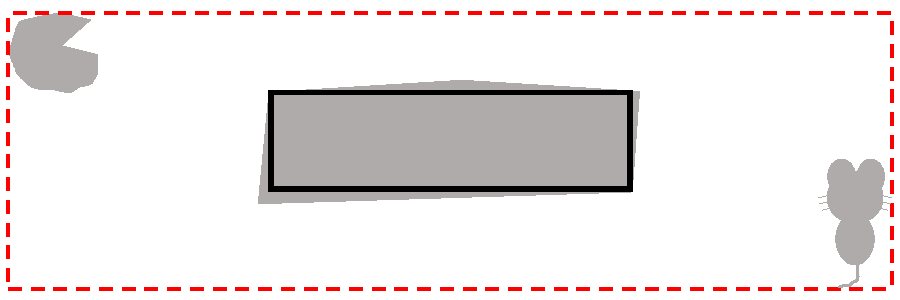
\includegraphics[width=3in]{fig.pdf}
\caption{Example where the underlying distribution $p$ is uniform over the (gray) valid regions. The solid rectangle maximizes our objective since it does not output nonsense (is supported only within the grey matter) and is closest to the $p$ (covers the maximum amount of grey matter). In contrast, the standard maximum likelihood (dashed red) rectangle must fully contain the observed samples, thus generating invalid points most of the time.  }
\end{figure}

Motivated by these observations, we evaluate a generative model $q$ on two axes. First is {\em coverage}, which is related to the probability assigned to future examples drawn from the true distribution $p$. Second is {\em validity}, defined as the probability that random examples generated from $q$ meet some validity requirement. Formally, we measure coverage in terms of a bounded {\em loss}:
$$\Loss(p,q)=\E_{x \sim p}[L(q_x)],$$
where $L:[0,1]\rightarrow [0,M]$ is a bounded decreasing function such as the capped log-loss $L(q_x)=\min(M, \log 1/q_x)$. % or $L(q_x)=\log 1/(q_x+\exp(-M))$. 
A bounded loss has the advantages of being efficiently estimable, and also it enables a model to assign 0 probability to one example (e.g., an outlier or error) if it greatly increases the likelihood of all other data. Validity is defined with respect to a set $V \subseteq X$, and $q(V)$ is the probability that a random example generated from $q$ lies within $V$. 

Clearly, there is a tradeoff between coverage and validity. We first focus on the case of (near) perfect validity. A Valid Generative Modeling (VGM) algorithm if it outputs, for a family of distributions $Q$ over $X$, if it outputs $\hat{q}$ with (nearly) perfect validity and whose loss is nearly as good as the loss of the best valid $q\in Q$. More precisely, $A$ is a VGM learner of $Q$ if for any nonempty valid subset $V \subseteq X$, any probability distribution $p$ over $V$, and any $\eps>0$, $A$ uses $n$ random samples from $p$ and makes $m$ membership oracle calls to $V$ and outputs a distribution $\hat{q}$ such that, $$\Loss(p, \hat{q}) \leq \min_{q \in Q: q(V)=1}\Loss(p,q) + \eps ~\text{ and }~\hat{q}(V)\geq 1-\eps.$$ 
We aim for our learner to be sample and query efficient, requiring that $n$ and $m$ are polynomial in $M, 1/\eps$ and a measure of complexity of our distribution class $Q$.
Furthermore, we would like our algorithms to be computationally efficient, with a runtime polynomial in the size of the data, namely the $n + m$ training examples. 
A more formal description of the problem is available in Section~\ref{sec:problem}.

$A$ is said to be {\em proper} if it always outputs $\hat{q}\in Q$ and {\em improper} otherwise.
In Section~\ref{sec:impossibility}, we first show that efficient proper learning for VGM is impossible. This is an information-theoretic result, meaning that even given infinite runtime and positive samples, one still cannot solve the VGM problem. Interestingly, this is different from binary classification, where it is possible to statistically learn from iid examples without a membership oracle.

Our first main positive result is an efficient (improper) learner for VGM. The algorithm relies on a subroutine that solves the following {\em Generative Modeling with Negatives} (GMN) problem: given sets $X_P, X_N \subset X$ of positive and negative examples, find the probability distribution $q \in Q$ which minimizes $\sum_{x \in X_P} L(q(x))$ subject to the constraint that $q(X_N)=0$. For simplicity, we present our algorithm for the case that the distribution family $Q$ is finite, giving sample and query complexity bounds that are logarithmic in terms of $|Q|$. However, as we show in Section~\ref{sec:infinite-families}, all of our results extend to infinite families $Q$. It follows that if one has a computationally efficient algorithm for the GMN problem for a distribution family $Q$, then our reduction gives a computationally efficient VGM learning algorithm for $Q$.

Our second positive result is an algorithm that minimizes $\Loss(p,q)$ subject to a relaxed validity constraint comparing against the optimal distribution that has validity $q(V)$ at least $1-\alpha$ for some $\alpha>0$. We show in Section~\ref{sec:partial-validity} that even in this more general setting, it is possible to obtain an algorithm that is statistically efficient but may not be computationally efficient. An important open question is whether there exists a computationally efficient algorithm for this problem when given access to an optimization oracle, as was the case for our algorithm for VGM.

\subsection{Related Work}
\cite{KearnsMRRSS94} showed how to learn distributions from positive examples in the realizable setting, i.e., where the true distribution is assumed to belong to the class being learned. In the same sense as their work is similar to PAC learning \citet{Valiant84} of distributions, our work is like agnostic learning \citet{KearnsSS94} in which no assumption on the true distribution is made. 

Generative Adversarial Networks (GANs)~\cite{GoodfellowPMXWOCB14} are an approach for generative modeling from positive examples alone, in which a generative model is trained against a discriminator that aims to distinguish real data from generated data. In some domains, GANs have been shown to outperform other methods at generating realistic-looking examples. Several shortcomings of GANs have been observed \citet{AroraRZ18}, and GANs are still subject to the theoretical limitations we argue are inherent to any model trained without a validity oracle. 

In supervised learning, there is a rich history of learning theory with various types of queries, including membership which are not unlike our (in)validity oracle. Under various assumptions, queries have been shown to facilitate the learning of complex classes such as finite automata \citet{Angluin88} and DNFs \citet{Jackson97}. See the survey of \cite{Angluin92} for further details.  Interestingly, \cite{Feldman09} has shown that for agnostic learning, i.e., without making assumptions on the generating distribution, the addition of membership queries does not enhance what is learnable beyond random examples alone. 
Supervised learning also has a large literature around active learning, showing how the ability to query examples reduces the sample complexity of many algorithms. See the survey of \cite{Hanneke14}. Note that the aim here is typically to save examples and not to expand what is learnable.
 
More sophisticated models, e.g., involving neural networks, can mitigate the invalidity problem as they often generate more realistic natural language and have even been demonstrated to generate \LaTeX{} that nearly compiles \citep{Karpathy15} or nearly valid Wikipedia markdown. However, longer strings generated are unlikely to be valid. For example, \cite{Karpathy15} shows generated markdown which includes:
\begin{quote}
==Access to ''rap===
The current history of the BGA has been [[Vatican Oriolean Diet]], British Armenian, published in 1893.  While actualistic such conditions such as the [[Style Mark Romanians]] are still nearly not the loss.
\end{quote}

Even ignoring the mismatched quotes and equal signs, note that this example has two so-called ``red links'' to two pages that do not exist. Without checking, it was not obvious to us whether or not Wikipedia had pages titled {\em Vatican Oriolean Diet} or {\em Style Mark Romanians}. In some applications, one may or may not want to disallow red links. In the case that they are considered valid, one may seek a full generative model of what might plausibly occur inside of brackets, as the neural network has learned in this case. If they are disallowed, a model might memorize links it has seen but not generate new ones. A validity oracle can help the learner identify what it should avoid generating.

 In practice, \cite{KusnerPH17} discuss how generative models from neural networks (in particular autoencoders) often generate invalid sequences. 
\cite{JanzWPKH18} learn the validity of examples output by a generative model using oracle feedback. 


\section{Preliminaries}
\label{sec:model}
\section{Property Testing Background and Models}
\label{sec:model}
\subsection{Query Testing (Standard Property Testing)}
Given functions $f$ and $g$ over domain $X$, we define the distance between $f$ and $g$ with respect to distribution $\calD$ over $X$ to be
\begin{equation}
\dist_\calD(f,g)=\Pr_{x\sim\calD}[f(x)\neq g(x)].
\end{equation}
Given a class $\calC$ of functions over domain $X$ and a margin $\epsilon$, a \emph{property tester} distinguishes the case that the input function $f$ is in the class $\calC$ from the case that $f$ is $\epsilon$-far from $\calC$:
\begin{enumerate}
\item if $f\in\calC$, the tester accepts $f$ with probability at least $\frac{2}{3}$;
\item if $\forall g\in\calC,\dist_\calD(f,g)>\epsilon$, the tester rejects $f$ with probability at least $\frac{2}{3}$.
\end{enumerate}
\citet{RS96} first studied the property testing model assuming $X$ is finite and $\calD$ is uniform. We call the testing model of \citet{RS96} as \emph{query testing}, because the tester makes queries to access $f$, i.e., the tester asks for the value of $f(x)$ for some $x\in X$ for each query it makes.

\citet{PRR06} first studied the \emph{tolerant} version of property testing: given an additional parameter, the threshold $\alpha$, to distinguish a function $\alpha$-close to the class from a function $(\alpha+\epsilon)$-far from the class. In other words, 
\begin{enumerate}
\item if $\exists g\in \calC,\dist_\calD(f,g)\leq\alpha$, the tester accepts $f$ with probability at least $\frac{2}{3}$;
\item if $\forall g\in\calC,\dist_\calD(f,g)>\alpha+\epsilon$, the tester rejects $f$ with probability at least $\frac{2}{3}$.
\end{enumerate}
They showed tolerant testers for clustering and for monotonicity in the query testing model. \citet{FF05} showed the existence of classes of binary functions that are efficiently query-testable in the non-tolerant case but are not efficiently query-testable in the tolerant case.

\citet{PRR06} also considered a similar task called distance approximation: estimating the distance from the function to the class so that with probability at least $\frac 23$ the output is within $\pm\epsilon$ to the true distance. Note that distance approximation with additive error $\epsilon$ implies tolerant testing with margin $2\epsilon$ with the same query complexity. Based on this observation, all the tolerant testers we design in this paper actually perform distance approximation (so we don't need the parameter $\alpha$) because distance approximation is a slightly more convenient model for our presentation.
\subsection{Passive Testing (Sample-Based Testing)}
\label{subsec:passive}
\citet{GGR98} first studied testers with the ability to obtain a random sample in addition to making queries so that the tester can potentially work on arbitrary distributions (see Section \ref{subsec:distributionfree} for distribution-free testing), although their algorithmic results remained in the query testing framework over the uniform distribution.
\citet{KR98} developed the first \emph{passive} testers, testers that don't make queries and only rely on the random i.i.d.\ sample to access the input function $f$, for a variety of classes with sub-learning sample complexity. \citet{GR13} advanced the study of passive testers by providing several general positive results as well as by revealing relations with other testing models.

\emph{Proper} learning implies testing, simply by testing using the output hypothesis, but passive testing can be substantially harder than \emph{improper} learning. \citet{GGR98} pointed out that the class of $k$-term-DNF is NP-hard for non-tolerant passive testing while it is efficiently PAC learnable via $k$-CNF \citep{PV88}, if we require testing and learning on an arbitrary distribution.

The general hardness of \emph{tolerant} passive testing based on hardness of improper \emph{agnostic} learning can be implied from the recent work by \citet{KL18}. They considered the task of refutation: for any fixed distribution $\calD$ over domain $X$, given a sample of example-label pairs $\{(x_i,y_i)\}$ and margin $\epsilon>0$, to distinguish the following two cases:
\begin{enumerate}
\item accept when every $(x_i,y_i)$ is i.i.d.\ from some distribution $\calD'$ over $X\times\{0,1\}$ with marginal on $X$ being $\calD$ and $\exists f\in\calC,\Pr_{(x,y)\sim\calD'}[f(x)\neq y]\leq\frac 12-\epsilon$;
\item reject when every $x_i$ is i.i.d.\ from $\calD$ and every $y_i$ is i.i.d.\ from the uniform distribution over $\{0,1\}$.
\end{enumerate}
They showed that a refutation algorithm for distribution $\calD$ with margin $\epsilon$ and sample complexity $s$ implies an improper agnostic learning algorithm for the same distribution with error $3\epsilon$ and sample complexity $O(\frac{s^3}{\epsilon^2})$. We show in Appendix \ref{sec:refutation} that the refutation algorithm can be reduced to a tolerant passive tester for arbitrary unknown distributions with threshold $\alpha=\frac 12-\frac{3\epsilon}4$, margin $\frac{\epsilon}{2}$, and sample complexity $\Omega(s)$, implying that tolerant passive testing for arbitrary unknown distributions can't be substantially more sample-efficient than improper agnostic learning for any distribution $\calD$ (with some reasonable assumptions about the distribution $\calD$). %The reduction also has a uniform-distribution version (Lemma \ref{}), implying the hardness of tolerant passive testing over the uniform distribution.

%\citet{Vad17} showed that if one can perform refutation, i.e., distinguishing a function in the class from a random function, using a sample of size $s$, then one can also do improper PAC learning with sample complexity $O(\poly(s))$.  \citet{KL18} showed similar results for the tolerant (agnostic) case. They used a different definition of refutation: distinguishing a function having distance $\frac 12-\epsilon$ to the class from a random function, and showed that if one can perform refutation using a sample of size $s(\epsilon)$, then one can also do improper agnostic learning with sample complexity $O(\frac{\left(s(\frac\epsilon 2)\right)^3}{\epsilon^2})$.\footnote{One difference between the two results is that \citet{Vad17} assumes that the distribution is arbitrary while the result by \citet{KL18} is distribution-specific. } Note that passive testing implies refutation with the same sample complexity both in the non-tolerant and the tolerant case, assuming the concept class has a finite VC-dimension and the distribution has no massive points so that a random function has distance $\frac 12$ to it with probability 1. Therefore these results imply that passive testing can't be substantially more sample-efficient than improper learning.

\subsection{Active Testing}
Both query testing and passive testing have shortcomings. The assumption of query testing that the tester can make queries to arbitrary points in the domain is usually impractical, while passive testing is too restrictive: for the tolerant case, passive testing can't be substantially more sample-efficient than agnostic learning (recall Section \ref{subsec:passive}).

To avoid both shortcomings, \citet{BBBY12} proposed the active testing model where the tester first receives an unlabeled random i.i.d.\ sample and then makes queries to points in the sample. While the size of the unlabeled sample might be comparable to the labeled sample complexity for learning, the number of queries the tester makes should be substantially smaller.
%large (but is still required to be polynomial in the VC-dimension of the class), the number of queries the tester makes should be substantially smaller than the sample complexity for learning. 
They showed (non-tolerant) active testers for unions of $d$ intervals and for linear separators.
\subsection{Distribution-Free Testing}
\label{subsec:distributionfree}
Distribution-free testing \citep{GGR98} considers testers that work on arbitrary unknown distributions with the ability to obtain random i.i.d.\ sample in addition to making queries. \citet{HK03} designed distribution-free testers for low-degree multivariate polynomials, monotone functions, and several other classes.

The difference between distribution-free testing and passive testing (over arbitrary unknown distributions) is that distribution-free testers have the ability to make queries while passive testers don't. However, the query ability is helpful only when we do \emph{non-tolerant} testing where the tester is only required to accept functions in the class, rather than functions having distance 0 to the class with respect to the unknown distribution. For \emph{tolerantly} testing binary functions, we show that distribution-free testing implies passive testing with the same sample complexity (see Section \ref{sec:relationship} Lemmas \ref{lm:distributionfreenontolerant} and \ref{lm:distributionfreetolerant}) and thus the hardness for tolerant passive testing extends automatically to tolerant distribution-free testing.



%\subsection{Property Testing, Tolerant Testing and Distance Approximation}
%Suppose we have a ground set $X$ and a distribution $\calD$ over $X$. For any two binary functions $f,g\in\{0,1\}^X$, we define their distance to be $\dist_{\calD}(f,g)=\Pr_{x\sim \calD}[f(x)\neq g(x)]$. 

%Suppose we also have a concept class $\calC\subseteq\{0,1\}^X$. Given a function $f\in\{0,1\}^X$ and a margin $\epsilon$ as input, the task of property testing $\pt_{\calD}(f,\epsilon)$ \citep{RS96} is to distinguish the case that $f$ belongs to class $\calC$ from the case that $f$ is $\epsilon$-far from $\calC$. In other words, $\forall f$,
%\begin{enumerate}
%\item if $f\in\calC$, the algorithm outputs ``YES'' with probability at least $\frac{2}{3}$;
%\item if $\forall g\in\calC,\dist_{\calD}(f,g)>\epsilon$, the algorithm outputs ``NO'' with probability at least $\frac{2}{3}$.
%\end{enumerate}
%A property testing algorithm may be randomized, and in this case, the goal is to output the correct answer with probability at least $\frac{2}{3}$. The success probability can be boosted to $1-\delta$ by repeating the algorithm for $O(\log\frac{1}{\delta})$ times and taking the majority.

%The function $f$ can be given to the algorithm in many different ways. In the \emph{query testing} framework \citep{RS96}, the algorithm can query the value of $f(x)$ for any $x\in X$. In this framework, we say the algorithm has \emph{query access} to $f$, or has access to $f\qu$. The query complexity of the algorithm, as a function of $\frac{1}{\epsilon}$, is measured by the maximum number of queries needed by the algorithm.

%\citet{BBBY12} argued that the query testing framework is not realistic for machine learning practice. They proposed the \emph{active testing} framework, in which the algorithm first requests $N$ unlabeled examples $x_1,x_2,\cdots,x_{N}\in X$ sampled independently according to $\calD$ and can only choose to query $f(x_i)$ for $1\leq i\leq N$. In this framework, we say the algorithm has \emph{active access} to $f$, or has access to $f\ac$. The maximum value of $N$, as a function of $\frac{1}{\epsilon}$, is called the \emph{unlabeled sample complexity}. The query complexity is still defined as a function of $\frac{1}{\epsilon}$ measuring the maximum number of queries needed by the algorithm.

%\citet{GGR98} and \citet{KR98} studied an even more strict way of accessing $f$, called \emph{passive access}, in which the algorithm is given the label of an example chosen independently at random from $\calD$ for each query the algorithm makes. 

%Tolerant testing $\tot_{\calD}(f,\alpha,\epsilon)$ \citep{PRR06} is a similar task to property testing. The only difference is that besides the margin $\epsilon$, we are given another parameter $\alpha$ as input, and we are asked to distinguish the case that $f$ is $\alpha$-close to $\calC$ from the case that $f$ is $(\alpha+\epsilon)$-far from $\calC$. %following two cases:
%\begin{enumerate}
%\item $\exists g\in\calC,\dist_{\calD}(f,g)\leq \alpha$;
%\item $\forall g\in\calC,\dist_{\calD}(f,g)>\alpha+\epsilon$.
%\end{enumerate} 
%The query complexity of tolerant testing is still measured as a function of $\frac{1}{\epsilon}$ \citep{PRR06}. 

%A natural generalization of tolerant testing is distance approximation, in which we are only given the function $f$ and the margin $\epsilon$ as input and required to output $\hat\alpha$ as an approximation of the distance from $f$ to $\calC$ up to an additive error $\epsilon$. More specifically, the goal of $\da_{\calD}(f,\epsilon)$ is to output $\hat\alpha$ such that $\forall f$,
%\begin{enumerate}
%\item $\forall \alpha$ such that $\exists g\in\calC,\dist_{\calD}(f,g)\leq \alpha$, it holds with probability at least $\frac{2}{3}$ that $\hat\alpha\leq \alpha+\epsilon$;
%\item $\forall \alpha$ such that $\forall g\in\calC,\dist_{\calD}(f,g)>\alpha$, it holds with probability at least $\frac{2}{3}$ that $\hat\alpha> \alpha-\epsilon$.
%\end{enumerate}

%The success probability of a distance approximation algorithm can be boosted to $1-\delta$ by repeating it $O(\log\frac{1}{\delta})$ times and taking the median. 

%Because for any $\calD$ and $\epsilon$, it's clear that a $\da_{\calD}(f,\frac{\epsilon}{2})$ algorithm implies a $\tot_{\calD}(f,\alpha,\epsilon)$ algorithm with the same query and unlabeled sample complexity \citep{PRR06}, we focus on distance approximation rather than tolerant testing throughout the paper.

%For all of the above examples, the distribution $\calD$ appears in the subscript meaning that the distribution is fixed and known to the algorithm. In this paper, we will consider a more general case, for example $\pt(f\qu,\epsilon,\calD)$, in which the distribution $\calD$ is arbitrarily given to the algorithm as input. When the algorithm has active or passive access to $f$, it's possible to consider an even more general case, for example $\pt(f\ac,\epsilon)$, in which the distribution $\calD$ is unknown to the algorithm (but implicitly given to the algorithm when accessing $f$).




%We use $q^{\text{query}}(\epsilon)$ and $q^{\text{active}}(\epsilon)$ to denote the maximum number of queries needed in the query testing model and the active testing model, respectively. \citet{BBBY12} showed that $q^{\text{query}}(\epsilon)\leq q^{\text{active}}(\epsilon)$ always holds for non-tolerant property testing, which can be easily generalized to tolerant testing and distance approximation. They also showed for non-tolerant property testing that when $\calC$ is the class of dictator functions and $\calD$ is the uniform distribution over $\{0,1\}^p$, there is a testing algorithm in the query testing framework whose query complexity $q^{\text{query}}(p,\epsilon)$ does not grow with respect to $p$, while every testing algorithm in the active testing framework requires $q^{\text{active}}(p,\epsilon)=\Omega(\log p)$ queries for any fixed $0<\epsilon<\frac{1}{2}$.

%In this paper, however, we will show in Theorem \ref{thm:unlabeled} a reversed inequality that $q^{\text{active}}(\epsilon)=O(q^{\text{query}}(\frac{\epsilon}{2}))$ when we are required to do testing on \emph{arbitrary} distribution $\calD$ and the queries are required to lie in the support of $\calD$ (when we have query access)\footnote{We can assume without loss of generality that the queries all lie in the support of $\calD$ when we do tolerant testing and distance approximation, but we cannot assume this for non-tolerant property testing. The reason is that $f\in\calC$ is stronger than $\exists g\in\calC,\dist_{\calD}(f,g)=0$.}, uncovering the relationship between query access and active access.


%Similar to Theorem \ref{thm:unlabeled}, we have the following theorem in tolerant testing. Its proof is a simple modification of the proof to Theorem \ref{thm:unlabeled}.






\section{Group Externality of Exploration}
\label{sec:negative}

In this section, we study the externalities of exploration at a group
level, quantifying how much the presence of one population impacts the
rewards of another in an online learning system. We consider linear
contextual bandits in a setting in which there are two underlying user
populations, called the \emph{majority} and the \emph{minority}. The
user who arrives at round $t$ is assumed to come from the majority
population with some fixed probability and the minority population
otherwise, and the population from which the user comes is known to
the learner. The tuple of context vectors at time $t$ is then drawn
independently from a fixed group-specific distribution.

We assume there is a
single hidden vector $\theta$, and that the distribution of rewards conditioned
on the chosen context vector is
the same for both groups. Only the distribution over tuples of
available context vectors differs between groups. This implies that
externalities cannot be explained by the absence of a good policy,
since there always exists a policy that is simultaneously optimal for
everyone. This allows us to focus only on externalities inherent to the
process of exploration.

We define the \emph{minority regret} to be the regret experienced by
the minority. The \emph{group
  externality} imposed on the minority by the majority is then the
difference between the minority regret of an algorithm run on the
minority alone and the minority regret of the same algorithm run on
the full population. A negative group externality implies that the
minority is worse off due to the presence of the majority.
It is generally more meaningful to bound the multiplicative
difference between the minority regret obtained with and without the
majority present. Several of our results have this form. \looseness=-1

We first ask whether large group externalities can exist. We show that
on a simple toy example, a large negative group externality arises
under LinUCB, while a slight variant of this example leads to a large
positive externality. Put another way, more available data can lead to
either better or worse outcomes for the users of a system. We show
that this general phenomenon is unavoidable. That is, no algorithm can
simultaneously approximate the minority regret of LinUCB run on the
full population and LinUCB run on the minority alone, up to any
$o(\sqrt{T})$ multiplicative factor.

\subsection{Two-Bridge Instance}
We consider a toy example, motivated by a scenario in which a learner
is choosing driving routes for two groups of users. Each user starts
at point $A$, $B$, or $C$, and wants to get to the same destination,
point $D$, which requires taking one of two bridges, as shown in
Figure~\ref{fig:bridges}. The travel costs for each of the two bridges
are unknown. For simplicity, assume all other edges are known to have
0 cost.

Suppose that 95\% of users are in the majority group. All of these
users start at point $A$ and have access only to the top bridge. The
other 5\% are in the minority. Of these users, 95\% start at point
$C$, from which they have access only to the bottom bridge. The
remaining 5\% of the minority users start at point $B$, and have
access to both bridges.

\begin{figure}
\centering
\begin{tikzpicture}[scale=.75]
\node[circle, draw] (A) at (-2,-1) {$A$};
\node[circle, draw] (B) at (-1,-2) {$B$};
\node[circle, draw] (C) at (-2,-3) {$C$};
\node[circle, draw] (s1) at (1,-1) {};
\node[circle, draw] (s2) at (1,-3) {};
\node[circle, draw] (e1) at (4,-1) {};
\node[circle, draw] (e2) at (4,-3) {};
\node[circle, draw] (D) at (6,-2) {$D$};
\draw[->,draw,>=stealth] (A) -- (s1);
\draw[->,draw,>=stealth] (B) -- (s1);
\draw[->,draw,>=stealth] (B) -- (s2);
\draw[->,draw,>=stealth] (C) -- (s2);
\draw[->,draw,>=stealth,very thick] (s1) -- (e1) node[midway,above] {$\theta_1$};
\draw[->,draw,>=stealth,very thick] (s2) -- (e2) node[midway,above] {$\theta_2$};
\draw[->,draw,>=stealth] (e1) -- (D);
\draw[->,draw,>=stealth] (e2) -- (D);
\end{tikzpicture}
\caption{Visual illustration of the two-bridge instance. \label{fig:bridges}}
\end{figure}

Consider the behavior of an algorithm that follows the principle of
optimism under uncertainty.  If run on the full user population, it
will quickly collect many observations of the commute time for the top
bridge since all users in the majority group must travel over the top
bridge.  It will collect relatively fewer observations of the commute
time over the bottom bridge.  Therefore, when the algorithm is faced
with a member of the minority population who starts at point $B$, the
algorithm will likely send this user over the bottom bridge in order
to collect more data and improve its estimate. \looseness=-1

If the same algorithm is instead run on the minority alone, it will
quickly collect many more observations of the commute time for the
bottom bridge relative to the top.
Now when the algorithm is faced with a user who starts
at point $B$, it will likely send her over the top bridge.

Which is better depends on which bridge has the longer commute time.
If the top bridge is the better option, then the presence of the
majority imposes a negative externality on the minority. If not, then
the presence of the majority helps. These two scenarios may be
difficult to distinguish.

This toy example can be formalized in the linear contextual bandits
framework. There are two underlying actions (the two bridges), but
these actions are not always available. To capture this, we define a
parameter vector $\theta$ in $[0, 1]^2$, with the two coordinates
$\theta_1$ and $\theta_2$ representing the expected rewards for taking
the top and bottom bridge respectively. (Though we motivated
the example in terms of costs, it can be expressed equivalently in
terms of rewards.) There are two possible context vectors:
$[1 ~ 0]\tran$ and $[0 ~ 1]\tran$. A user has available an action with
context vector $[1 ~ 0]\tran$ if and only if she has access to the top
bridge. Similarly, she has available an action with context vector
$[0 ~ 1]\tran$ if and only if she has access to the bottom bridge. The
instance can then be formalized as follows.



\begin{definition}[Two-Bridge Instance]
  The \emph{two-bridge instance} is an instance of linear contextual
  bandits. On each round $t$, the user who arrives is from the
  majority population with probability 0.95, in which case
  $x_{1, t} = x_{2, t} = [1 ~ 0]\tran$. Otherwise, the user is in the
  minority. In this case, with probability 0.95,
  $x_{1,t} = x_{2,t} = [0 ~ 1]\tran$ (based on
  Figure~\ref{fig:bridges}, we call these $C$ rounds), while with probability 0.05, $x_{1,t} = [1 ~ 0]\tran$ and
  $x_{2,t} = [0 ~ 1]\tran$ ($B$ rounds). We consider two
  values for the hidden parameter vector $\theta$,
  $\thetazero = [1/2 \ ~ 1/2 - \varepsilon]\tran$ and
  $\thetaone = [1/2 - \varepsilon \ ~ 1/2]\tran$ where
  $\varepsilon = 1/\sqrt{T}$.
\end{definition}


\subsection{Performance of LinUCB}


We start by analyzing the performance of LinUCB on the two-bridge
instance.  Our main result formalizes the intuition above, showing
that when $\theta = \thetazero$ (that is, the top bridge is better)
the majority imposes a large negative group externality on the
minority, while the majority imposes a large positive externality when
$\theta = \thetaone$. We assume rewards are $1$-subgaussian.%
\footnote{A random variable $X$ is called $\sigma$-subgaussian if $E[e^{\sigma X^2}]<\infty$. A special case is Gaussians with variance $\sigma^2$.}


\begin{theorem}
  Consider LinUCB with any interval width function $f$ satisfying
  $f(t) \ge 2\sqrt{\log(T)}$.%
  \footnote{For instance, the interval width function in Equation~\eqref{eq:Abbasi-f} satisfies this condition whenever $d c_0\geq 4$, so one can either set $c_0\geq 2$, or add two more dimensions to the problem instance (and set $\theta_3 = \theta_4 =0$).}
   On the two-bridge instance,
  assuming $1$-subgaussian noise on the rewards, when
  $\theta = \thetazero$, LinUCB achieves expected minority regret
  $O(1)$
  when run on the minority alone, but $\Omega(\sqrt{T})$ when run on
  the full population.  In contrast, when $\theta = \thetaone$, LinUCB
  achieves expected minority regret $O(1)$ when run on the full
  population, but $\Omega(\sqrt{T})$ when run on the minority alone.
\label{thm:twobridgelinucb}
\end{theorem}

We omit the proofs of the $\Omega(\sqrt{T})$ lower bounds, which both
follow a similar structure to the one used in the proof of the general
impossibility result in Section~\ref{sec:impossibility}; in fact, both
of these lower bounds could be stated as an immediate corollary of
Theorem~\ref{thm:indistinguishability}.  Essentially, an argument
based on KL-divergence shows that it is difficult to distinguish
between the case in which $\theta = \thetazero$ and the case in which
$\theta = \thetaone$, and therefore LinUCB must choose similar actions
in these two cases.

To prove the $O(1)$ upper bounds, we make heavy use of the special
structure of the two-bridge instance, which significantly simplifies
the analysis of LinUCB. We exploit the fact that the only context
vectors available to the learner are the basis vectors $[1 ~ 0]\tran$
and $[0 ~ 1]\tran$, which essentially makes this an instance of
sleeping bandits~\citep{SleepingBandits-ml10}. In this special case,
the covariance matrix $Z_t$ is always diagonal, which simplifies
Equation~\eqref{eq:linucb_def} and leads to LinUCB choosing the $i$th
basis, where $i$ maximizes $(\thetahatt)_i + f(t)/\sqrt{(Z_t)_{ii}}$ and
$(Z_t)_{ii}$ is simply the number of times that this basis vector was
already chosen. Additionally, in this setting $(\thetahatt)_i$ is just the
average reward observed for the $i$th basis vector, allowing us to
bound the difference between each $(\thetahatt)_i$ and $\theta_i$ using
standard concentration techniques. Using this, we show that with high
probability, after a logarithmic number of rounds---during which the
learner can amass at most $O(1)$ regret since the worst-case regret on
any round is $\varepsilon = 1/\sqrt{T}$---the probability that LinUCB
chooses the wrong action on a $B$ round is small ($O(1/\sqrt{T})$).
This leads to constant regret on expectation.



\subsection{An Impossibility Result}
\label{sec:impossibility}

It is natural to ask whether it is possible to design an algorithm
that can distinguish between the two scenarios analyzed above,
obtaining minority regret that is close to the best of LinUCB run on
the minority alone and LinUCB run on the full population on any
problem instance. In this section, we show that the answer is no. In
particular, we prove that on the two-bridge instance, if
$\Pr[\theta = \thetazero] = \Pr[\theta = \thetaone] = 1/2$, then any
algorithm must suffer $\Omega(\sqrt{T})$ regret on expectation (and
therefore $\Omega(\sqrt{T})$ minority regret, since all regret is
incurred by minority users).

To prove this result, we begin by formalizing the idea that it is hard
to distinguish between the case in which $\theta = \thetazero$ and the
case in which $\theta = \thetaone$. To do so, we bound the
KL-divergence between the joint distributions over the sequences of
context vectors, actions taken by the given algorithm, and the given
algorithm's rewards that are induced by the two choices of $\theta$.
By applying the high-probability Pinsker lemma~\citep{T09}, we show
that a low KL-divergence between these distributions implies that the
algorithm must be likely either to choose the top bridge on $B$ rounds
more than half the time when the bottom bridge is better or to choose the
bottom bridge on $B$ rounds more than half the time when the top
bridge is better, either of which would lead to high
($\Omega(\sqrt{T})$) regret as long as the number of $B$ rounds is
sufficiently large. To finish the proof, we use a simple Chernoff
bound to show that the number of $B$ rounds is large with high
probability.

To derive the KL-divergence bound, we make use of the assumption that
the realized rewards $r_t$ at each round are either $0$ or $1$.  This
assumption is not strictly necessary.  An analogous argument could be
made, for instance, for real-valued rewards with Gaussian noise.

\begin{theorem} \label{thm:indistinguishability}
On the two-bridge instance with realized rewards $r_t \in \{0,1\}$, any algorithm must incur $\Omega(\sqrt{T})$ minority regret
in expectation when $\Pr[\theta = \thetazero] = \Pr[\theta = \thetaone] = \tfrac12$.
\end{theorem}

Note that ``any algorithm'' here includes algorithms run on the
minority alone, essentially ignoring data from the majority.
Theorems~\ref{thm:twobridgelinucb} and~\ref{thm:indistinguishability}
immediately imply the following corollary.

\begin{corollary}
No algorithm can simultaneously approximate the minority regret of both LinUCB run on the minority and LinUCB run on the full population up to any $o(\sqrt{T})$ multiplicative factor.
\end{corollary}


\section{Greedy Algorithms with Perturbed Contexts}
\label{sec:bayesian_greedy}
We now turn our attention to externalities at an individual level. We interpret exploration as a potential externality imposed on the current user of a system by future users, since the current user would prefer the learner to take the action that appears optimal.  One could avoid such externalities by running the greedy algorithm, which does just that, but it is well known that the greedy algorithm performs poorly in the worst case.  In this section, we build on a recent line of work analyzing the conditions under which inherent data diversity leads the greedy algorithm to perform well.

We analyze the expected performance of the greedy algorithm under small random perturbations of the context vectors. We focus on greedy algorithms that consume new data in batches, rather than every round. We consider both Bayesian and frequentist versions, \bg and \fg. Our main result is that for any specific problem instance, both algorithms match the Bayesian regret of any algorithm on that particular instance up to polylogarithmic factors. We also prove that under the same perturbation assumptions, LinUCB achieves regret $\tilde{O}(T^{1/3})$ for each realization of $\theta$, which implies a worst-case Bayesian regret of $\tilde{O}(T^{1/3})$ for the greedy algorithms. Finally, we repurpose our analysis to derive a positive result in the group setting, implying that the impossibility result of Section~\ref{sec:impossibility} breaks down when the data is sufficiently diverse.

\xhdr{Setting and notation.}
We consider a Bayesian version of linear contextual bandits, with 
$\theta$ drawn from a known
multivariate Gaussian prior
    $\prior = \mc N(\pmt, \pvt)$,
with $\pmt \in \R^d$ and invertible $\pvt \in \R^{d\times d}$.


To capture the idea of data diversity, we assume the context vectors on each round $t$ are generated using the following \emph{perturbed context generation} process:  First, a tuple $(\mu_{1,t} \LDOTS \mu_{K,t} )$ of \emph{mean context vectors} is drawn independently from some fixed distribution $\D_\mu$ over $(\R\cup \{\perp\})^K$, where $\mu_{a, t} = \perp$ means action $a$ is not available. For each available action $a$, the context vector is then $x_{a,t} = \mu_{a,t} + \varepsilon_{a, t}$, where $\varepsilon_{a, t}$ is a vector of random noise. Each component of
    $\varepsilon_{a, t}$
is drawn independently from a zero-mean Gaussian with standard deviation $\rho$.
We refer to $\rho$ as the \emph{perturbation size}. In general, our regret bounds deteriorate if $\rho$ is very small.
Together we refer to a distribution $\D_\mu$, prior $\prior$, and perturbation size $\rho$ as a \textit{problem instance}.

We make several technical assumptions. First, the distribution $\D_\mu$ is such that each context vector has bounded $2$-norm, i.e., $\|\mu_{a,t}\|_2 \le 1$. It can be arbitrary otherwise. Second, the perturbation size needs to be sufficiently small,  $\rho\leq 1/\sqrt{d}$.
Third, the realized reward $r_{a,t}$ for each action $a$ and round $t$ is
    $r_{a,t} = x_{a,t}\tran \theta + \eta_{a,t}$,
the mean reward $x_{a,t}\tran \theta$ plus standard Gaussian noise $\eta_{a,t}\sim \mc N(0, 1)$.\footnote{Our analysis can be easily extended to handle reward noise of fixed variance, i.e.,
    $\eta_{a,t}\sim \mc N(0, \sigma^2)$.
\fg would not need to know $\sigma$. \bg would need to know either $\Sigma$ and $\sigma$ or just $\Sigma/\ \sigma^2$.}

The history up to round $t$ is denoted by the tuple $h_t = ((x_{1}, r_1) \LDOTS (x_t, r_t))$.

\xhdr{The greedy algorithms.}
For the batch version of the greedy algorithm, time is divided in batches of $Y$ consecutive rounds each. When forming its estimate of the optimal action at round $t$, the algorithm may only use the history up to the last round of the previous batch, denoted $t_0$.

\bg forms a posterior over $\theta$ using prior $\prior$ and history $h_{t_0}$.  In round $t$ it chooses the action that maximizes reward in expectation over this posterior. This is equivalent to choosing
\begin{align}\label{eq:BG-est-defn}
 a_t = \argmax_a  x_{a,t}\tran \, \bmt, \quad
    \text{where $\bmt := \Exp[\theta \mid h_{t_0}] $ }.
\end{align}

\fg~does not rely on any knowledge of the prior. It chooses the best action according to the least squares estimate of $\theta$, denoted $\fmt$, computed with respect to history $h_{t_0}$:
\begin{align}\label{eq:FG-est-defn}
 \textstyle a_t = \argmax_a  x_{a, t}\tran \, \fmt, \quad
\text{where $\fmt = \argmin_{\theta'} \sum_{\tau = 1}^{t_0} ((\theta') \tran
x_{\tau} - r_{\tau})^2$}.
\end{align}

\subsection{Main Results}

We first state our main results before describing the intuition behind them. We  state  each theorem  in terms of the main relevant parameters $T$, $K$, $d$, $Y$, and $\rho$.
First, we prove that in expectation over the random perturbations, both greedy algorithms favorably compare to any other algorithm.

\begin{theorem}
With perturbed context generation, there is some
  $Y_0 = \polylog(d, T)/\rho^2$
such that with batch duration $Y\geq Y_0$, the following holds. Fix any bandit algorithm, and let $R_0(T)$ be its Bayesian regret on a particular problem instance. Then on that same instance,
\begin{OneLiners}
\item[(a)] \bg has Bayesian regret at most
    $Y \cdot R_0(T/Y) + \tilde O(1/T)$,
\item[(b)]\fg has Bayesian regret at most
    $Y \cdot R_0(T/Y) + \tilde O(\sqrt{d}/\rho^2).$
\end{OneLiners}
\label{thm:main-greedy}
\end{theorem}

Our next result asserts that the Bayesian regret for LinUCB and both greedy algorithms is on the order of (at most) $T^{1/3}$. This result requires additional technical assumptions.

\begin{theorem}
Assume that the maximal eigenvalue of the covariance matrix $\Sigma$ of the prior $\prior$ is at most $1$,%
\footnote{In particular, if $\prior$ is independent across the coordinates of
$\theta$, then the variance in each coordinate is at most $1$.}
and the mean vector satisfies
    $\|\pmt\|_2\geq 1+\sqrt{3 \log T} $.
With perturbed context generation,
\begin{OneLiners}
\item[(a)] With appropriate parameter settings, LinUCB has Bayesian regret
    $\tilde O(d^2\,K^{2/3}\;T^{1/3}/\rho^2)$.
\item[(b)]If $Y\geq Y_0$ as in Theorem~\ref{thm:main-greedy}, then both \bg and \fg have Bayesian regret at most
    $\tilde O(d^2\,K^{2/3}\;T^{1/3}/\rho^2)$.
\end{OneLiners}
\label{thm:main-worst-case}
\end{theorem}

The assumption $\|\pmt\|_2\geq 1+\sqrt{3 \log T} $ in Theorem~\ref{thm:main-worst-case} can be replaced with $d \ge \log T/\log \log T$.
We use Theorem~\ref{thm:main-worst-case}(b) to derive an ``approximately prior-independent" result for \fg. (For clarity, we state it for independent priors.) The bound in Theorem~\ref{thm:main-worst-case}(b) deteriorates if $\prior$ gets very sharp, but it suffices if $\prior$ has standard deviation on the order of (at least) $T^{-2/3}$.

\begin{corollary}
Assume that the prior $\prior$ is independent over the components of $\theta$, with variance $\kappa^2\leq 1$ in each component. Suppose the mean vector satisfies
    $\|\pmt\|_2\geq 1+\sqrt{3 \log T} $.
With perturbed context generation, if $Y\geq Y_0$ as in Theorem~\ref{thm:main-greedy}, then \fg has Bayesian regret at most
    $\tilde O(d^2\,K^{2/3}\;T^{1/3}/\rho^2)$
as long as $\kappa\geq T^{-2/3}$.
\label{cor:sharp-priors}
\end{corollary}

Finally, we derive a positive result on group externalities. We find that with perturbed context generation, the minority Bayesian regret of the greedy algorithms (i.e., the Bayesian regret incurred on minority rounds) is small compared to the minority Bayesian regret of any algorithm, whether run on the full population \emph{or} on the minority alone. This sidesteps the impossibility result of Section~\ref{sec:impossibility}.

\begin{theorem}
Assume $Y\geq Y_0$ as in Theorem~\ref{thm:main-greedy} and perturbed context generation. Fix any bandit algorithm and instance, and let $R_{\min}(T)$ be the minimum of its minority Bayesian regrets when it is only run over minority rounds or when it is run over the full population. Both greedy algorithms run on the full population achieve minority Bayesian regret at most
    $Y\cdot R_{\min}(T) + \tilde O(\sqrt{d}/\rho^2)$.
  \label{thm:main-greedy-externalities}
\end{theorem}

\subsection{Key Techniques}
\label{sec:bayesian_greedy-key}

The key idea behind our approach is to show that, with perturbed context generation, \BayesGreedy collects data that is informative enough to
``simulate'' the history of contexts and rewards from the run of any other algorithm ALG over fewer rounds. This implies that it remains competitive with ALG since it has at least as much information and makes myopically optimal decisions. \looseness=-1

We use the same technique to prove a similar simulation result for \FreqGreedy. To treat both algorithms at once, we define a template that unifies them. A bandit algorithm is called \emph{\GreedyStyle} if it divides the timeline in batches of Y consecutive rounds each, in each round $t$ chooses some estimate $\theta_t$ of $\theta$, based only on the data from the previous batches, and then chooses the best action according to this estimate, so that
   $a_t = \argmax_a \theta_t\tran x_{a,t}$.
 For a batch that starts at round $t_0+1$, the \emph{batch history} is the tuple
 $((x_{t_0+\tau},\,r_{t_0+\tau}):\; \tau\in [Y])$,
 and the \emph{batch context matrix} is the matrix $X$ whose rows are vectors
 $(x_{t_0+\tau}:\; \tau\in [Y])$;
 here $[Y] = \{1, \cdots, Y\}$. Similarly to the ``empirical covariance matrix",
 we define the \emph{batch covariance matrix} as $X\tran X$.

Let us formulate what we mean by ``simulation". We want to use the data collected from a single batch in order to simulate the reward for any one context $x$. More formally, we are interested in the randomized function that takes a context $x$ and outputs an independent random sample from $\mathcal{N}(\theta\tran x, 1)$. We denote it $\Rew(\cdot)$; this is the realized reward for an action with context vector $x$.



\begin{definition}
Consider batch $B$ in the execution of a \GreedyStyle algorithm. Batch history $h_B$ can simulate $\Rew()$ up to radius $R>0$ if there exists a function
    $g: \{\text{context vectors}\}\times \{ \text{batch histories $h_B$}\} \to \R$
such that $g(x,h_B)$ is identically distributed to $\Rew(x)$ conditional on the batch context matrix, for all $\theta$ and all context vectors $x\in \R^d$ with $\|x\|_2\leq R$.
\label{def:simulation}
\end{definition}

Let us comment on how it may be possible to simulate $\Rew(x)$. For intuition, suppose that
    $x = \tfrac12\, x_1 + \tfrac12\, x_2$.
Then $(\tfrac12\, r_1 + \tfrac12\, r_2 + \xi)$ is distributed
as $\mathcal{N}(\theta\tran x, 1)$ if $\xi$ is drawn independently
from $\mathcal{N}(0, \tfrac12)$. Thus, we can define
    $g(x,h) = \tfrac12\, r_1 + \tfrac12\, r_2 + \xi$
in Definition~\ref{def:simulation}. We generalize this idea and
show that a batch history can simulate $\Rew$ as long as the batch covariance
matrix
has a sufficiently
large minimum eigenvalue, which holds with high probability
when the batch size is large. \looseness=-1


\begin{lemma}
 With perturbed context generation,
  there is some $Y_0 = \polylog(d, T)/\rho^2$ and
  $R = O(\rho \sqrt{d\log(TKd)}) $ such that with probability at least
  $1-T^{-2}$ any batch history from a
  \GreedyStyle algorithm can
    simulate $\Rew()$ up to radius $R$, as long as
    $Y\geq Y_0$.
    \label{lem:simulation}
\end{lemma}

If the batch history of an algorithm can simulate $\Rew$, the algorithm has enough information to simulate the outcome of a fresh round of any other algorithm
$\ALG$. Eventually, this allows us to use a coupling argument in which
we couple a run of \bg with a slowed-down run of $\ALG$, and prove
that the former accumulates at least as much information as the
latter, and therefore the Bayesian-greedy action choice is, in
expectation, at least as good as that of $\ALG$. This leads to
Theorem~\ref{thm:main-greedy}(a). We extend this argument to a
scenario in which both the greedy algorithm and $\ALG$ measure regret
over a randomly chosen subset of the rounds, which leads to
Theorem~\ref{thm:main-greedy-externalities}.

To extend these results to \fg, we consider a hypothetical algorithm that receives the same data as \fg, but chooses actions based on the (batched) Bayesian-greedy selection rule. We analyze this hypothetical algorithm using the same technique as above, and then argue that its Bayesian regret cannot be much smaller than that of \fg. Intuitively, this is because the two algorithms form
almost identical estimates of $\theta$, differing only in the fact that the hypothetical algorithm uses the $\prior$ as well as the data. We show that this difference amounts to effects on the order of $1/t$, which add up to a maximal difference of $O(\log T)$ in Bayesian regret.


\acks{We thank Solon Barocas, Dylan Foster, Jon Kleinberg, Aaron Roth, and Hanna Wallach for helpful discussions about these topics.}
\bibliography{refs}

\appendix

\section{Proof of Theorem~\ref{thm:twobridgelinucb} in Section~\ref{sec:negative}}

In this section, we prove that LinUCB achieves constant expected
minority regret when run on the minority alone with
$\theta = \thetazero$. The analysis of the expected minority regret of
LinUCB on the full population for $\theta = \thetaone$ is completely
analogous. We omit formal proofs of the $\Omega(\sqrt{T})$ lower
bounds, which follow a similar structure to the one used in the proof
of the general impossibility result in
Section~\ref{sec:impossibility}, and in fact would follow immediately
as a corollary of this result.

The proof makes use of the following concentration bound:


\begin{lemma} \label{lem:badrounds}
Let $C_t$ be the number of $C$ rounds observed in the first $t$ minority rounds
in the two-bridge instance. For any $\delta \in (0, 1)$,
with probability at least $1-\delta$, $C_t \ge 0.9t$ for all $t \ge 760 \log
(T/\delta)$.
\end{lemma}
\begin{proof}
We apply the following form of the Chernoff bound:
\[
  \Pr\b{C_t \le (1-\gamma) \E{C_t}} \le \exp\p{-\frac{\gamma^2}{2} \E{C_t}}.
\]
Setting $\gamma = 1/19$, we get
\begin{align*}
  \Pr\b{C_t \le \frac{9}{10}t} &=
  \Pr\b{C_t \le \p{1 - \frac{1}{19}} \frac{19}{20}t}
  \le \exp\p{-\frac{(1/19)^2}{2} \frac{19}{20} t}
  = \exp\p{-\frac{t}{760}}
  \le \frac{\delta}{T}
\end{align*}
for $t \ge 760 \log (T/\delta)$. Applying a union bound over all $T$ rounds, we have $C_t
\ge 0.9t$ for all $t \ge 760 \log(T/\delta)$ with probability at least
$1-\delta$.
\end{proof}

Now, consider LinUCB run on the minority population alone on the
two-bridge instance with $\theta = \thetazero$. Since we are
considering running LinUCB on the minority only, majority rounds are
irrelevant, so throughout this proof we abuse notation and use
$t \in \{1, \cdots, T_0\}$ for some $T_0 \leq T$ to index minority
rounds. $T$ is still the total number of (minority plus majority)
rounds.

  This proof heavily exploits the special structure of the two-bridge
  instance to simplify the analysis of LinUCB.  In particular, we
  exploit the fact that the only contexts ever available are the basis
  vectors $[1 ~ 0]\tran$ and $[0 ~ 1]\tran$.  This implies that the
  covariance matrix $Z_t$ is always diagonal, which greatly simplifies
  the expression for the chosen action in
  Equation~\eqref{eq:linucb_def}.  The optimistic estimate of the
  reward for choosing the $i$th basis vector is simply
  \begin{align}
    UCB_i^t := (\thetahatt)_i + f(t)/\sqrt{(Z_t)_{ii}} .
    \label{eq:ucbdef}
  \end{align}
  Additionally, in this special case,  $(Z_t)_{ii}$ is simply the
  number of times that the $i$th basis vector was chosen over the
  first $t$ minority rounds, and $(\thetahatt)_i$ is the average reward
  observed over the $(Z_t)_{ii}$ rounds on which it was chosen.

  Using this fact, we can apply concentration bounds to bound the
  difference between each $(\thetahatt)_i$ and $\theta_i$. Since rewards
  were assumed to be $1$-subgaussian,
  Lemma~\ref{lem:hoeffding} and a union bound give us that for any
  $\delta_1$, for any $t$, with probability at least $1-4\delta_1$, for all $i
  \in \{1,2\}$,
  \begin{align}
    \left\vert \theta_i - \thetahatti \right\vert \le
        \sqrt{2 \log (\tfrac{1}{\delta_1})/(Z_t)_{ii}}
  \label{eq:ucbbound}
\end{align}

Let $B_t$ and $C_t$ be the number of $B$ and $C$ rounds respectively
before round $t$. By Lemma~\ref{lem:badrounds}, for any $\delta_2$,
with probability $1-\delta_2$, $C_t \ge 9 B_t$ when
$t \ge 760 \log(T/\delta_2)$.  Suppose this is the case.  Since it is
only possible to choose $[1 ~ 0]$ on $B$ rounds, we have
$(Z_t)_{11} \leq B_T$. Similarly, since the algorithm can only choose
$[0 ~ 1]$ on every $C$ round, $(Z_t)_{22} \geq C_T \geq 9 B_T$.
Fixing $\delta_1 = 1/\sqrt{T}$ and using the assumption that
$f(t) \geq 2\sqrt{\log(T)}$, Equations~\eqref{eq:ucbdef}
and~\eqref{eq:ucbbound} then imply that for any $t \geq 760
\log(T/\delta_2)$, with probability at least $1-2\delta_1 = 1 -2\sqrt{T}$,
\begin{align*}
  UCB_1^{t}
  &\ge \theta_1 - \sqrt{\frac{2 \log (\sqrt T)}{(Z_t)_{11}}}+
  \frac{f(t)}{\sqrt{(Z_t)_{11}}}
  \ge \frac{1}{2} + \frac{1}{2}\frac{f(t)}{\sqrt{B_t}} ,
\end{align*}
and similarly,
\begin{align*}
  UCB_2^{t}
  &\le \theta_2 + \sqrt{\frac{2 \log (\sqrt{T})}{(Z_t)_{22}}} +
  \frac{f(t)}{\sqrt{(Z_t)_{22}}}
 \le \frac{1}{2} - \varepsilon   +\frac{3}{2}\frac{f(t)}{\sqrt{C_T}}
\le  \frac{1}{2} +\frac{1}{2}\frac{f(t)}{\sqrt{B_T}} \leq UCB_1^{t}.
\end{align*}


This shows that with probability at least $1-\delta_2$, after the
first $760 \log (T/\delta_2)$ rounds, LinUCB picks $[1 ~ 0]\tran$ on
each $B$ round with probability at least $1-2\delta_1$, leading to
zero regret on that round.  To turn this into a bound on expected
regret, first note that with at most $\delta_2$ probability, the
argument above fails to hold, in which case the minority regret is
still bounded by $\varepsilon B_T \leq \varepsilon T$.  When the argument
above holds, LinUCB may suffer up to $\varepsilon$ regret on each of the
first $760 \log (T/\delta_2)$ minority rounds.  On each additional
round, there is a failure probability of $2\delta_1$, and in this case
LinUCB again suffers regret of at most $\varepsilon$.  Putting this
together and setting $\delta_2 = 1/\sqrt{T}$, we get that the expected
regret is bounded by
$\delta_2 \varepsilon T
+ 760 \log(T/\delta_2) \varepsilon
+ 4\delta_1 \varepsilon T
= O(1)$.

\section{Proof of Theorem~\ref{thm:indistinguishability} in Section~\ref{sec:negative}}

  Fix any algorithm $\mathcal{A}$. We will first derive an
  $\Omega(\sqrt{T})$ lower bound on the expected regret of
  $\mathcal{A}$ conditioned on the number of
  $B$ rounds, $B_T$, being large. To complete the proof, we then show
  that $B_T$ is large
  with high probability.

  Let $h_t = \{(x_{1,\tau}, x_{2,\tau}, a_\tau, r_\tau)\}_{\tau=1}^t$ be a
  history of all context vectors, chosen actions, and rewards up to
  round $t$, with $h_0 = \emptyset$. Running $\mathcal{A}$ on the
  two-bridge instance with $\theta = \thetazero$ induces a
  distribution over histories $h_T$. Let $P$ denote the conditional
  distribution of these histories, conditioned on the event that $B_T
  \geq T/800$.  That is, we define
\[
P(h_T) := \Pr\left[h_T \left\vert \theta = \thetazero, B_T \geq
    T/800 \right.\right].
\]
  Similarly, we define
\[
Q(h_T) := \Pr\left[h_T \left\vert \theta = \thetaone, B_T \geq
    T/800 \right.\right].
\]

We first show that $\kl{P(h_T)}{Q(h_T)}$ is upper bounded a constant
that does not depend on $T$.
By the
  chain rule for KL divergences, since $r_t$ is independent of any
  previous contexts, actions, or rewards conditioned on $x_t$,
\begin{align*}
  \kl{P(h_T)}{Q(h_T)}
   =
  & \sum_{t=1}^T \Exp_{h_{t-1} \sim P}[\kl{P((x_{1,t}, x_{2,t}, a_t) \given
    h_{t-1})}{Q((x_{1,t}, x_{2,t}, a_t) \given h_{t-1})}] \\
  & + \sum_{t=1}^T \Exp_{(x_{1,t}, x_{2,t}, a_t) \sim P} [\kl{P(r_t \given x_{1,t}, x_{2,t}, a_t)}{Q(r_t
    \given (x_{1,t}, x_{2,t}, a_t))}] .
\end{align*}
Since the choice of context vectors available at time $t$ is
independent of the value of the parameter $\theta$ and $\mathcal{A}$
may only base its choices on the observed history and current choice
of contexts, it is always the case that
$P((x_{1,t}, x_{2,t}, a_t) \given h_{t-1}) = Q((x_{1,t}, x_{2,t}, a_t)
\given h_{t-1})$, so the first sum in this expression is equal to 0.

To bound the second sum, we make use of the assumption that
$r_t \in \{0,1\}$ for all $t$.\footnote{If we instead assumed rewards
  had Gaussian noise with variance $\sigma^2$, we would have
  $\kl{P_t(r_t \given x_{1,t}, x_{2,t}, a_t)}{Q_t(r_t \given x_{1,t}, x_{2,t}, a_t)} =
  \varepsilon^2/(2\sigma^2)$, and the proof would
  still go through.} Lemma~\ref{lem:bern_kl} then tells us that for
any round $t$,
$\kl{P(r_t \given x_{1,t}, x_{2,t}, a_t)}{Q(r_t \given x_{1,t}, x_{2,t}, a_t)} \le 7 \varepsilon^2/2$
since the probability of getting reward 1 conditioned on a chosen
context is always either $1/2$ or $1/2 - \varepsilon$. Putting this
together, we get that \[
  \kl{P(h_T)}{Q(h_T)} \le \frac{7\varepsilon^2 T}{2} = \frac{7}{2}.
\]

Now, let $E$ be the event that the algorithm $\mathcal{A}$ chooses arm
2 on at least half of the $B$ rounds, conditioned on $B_T \ge T/800$. If $E$ occurs when
$\theta = \thetazero$, the regret of $\mathcal{A}$ is at least
$B_T \varepsilon / 2$, which is on the order of $\sqrt{T}$ when
$B_T \geq T /800$. If $E$ does not occur (i.e., $\overline{E}$ occurs)
when $\theta = \thetaone$, $\mathcal{A}$ again has regret at least
$B_T \varepsilon / 2$. We will use the bound on KL
divergence to show that one of these bad cases happens with high
probability.

By Lemma~\ref{lem:pinkser},
\[
  P(E) + Q(\overline{E}) \ge \frac{1}{2} e^{-\kl{P(h_T)}{Q(h_T)}} \geq
  \frac{1}{2} e^{-7/2}.
\]

Let $R$ be the regret of $\mathcal{A}$.  We then have that
\begin{align*}
\Exp\left[R \left\vert B_T \geq \frac{T}{800}\right. \right] &= \frac{1}{2} \Exp\left[R \left\vert \theta = \thetazero, B_T \geq \frac{T}{800}\right. \right]
+ \frac{1}{2} \Exp\left[R \left\vert \theta = \thetaone, B_T \geq \frac{T}{800}\right. \right] \\
&\geq \frac{1}{2} \Pr\left[E \left\vert \theta = \thetazero, B_T \geq \frac{T}{800}\right. \right]
  \Exp\left[R \left\vert E, \theta = \thetazero, B_T \geq \frac{T}{800}\right. \right] \\
& \quad + \frac{1}{2} \Pr\left[\overline{E} \left\vert \theta = \thetaone, B_T \geq \frac{T}{800}\right. \right]
  \Exp\left[R \left\vert \overline{E}, \theta = \thetazero, B_T \geq \frac{T}{800}\right. \right] \\
&\geq \frac{1}{2} \left(P(E) + Q(\overline{E})\right) \frac{\sqrt{T}}{1600} \\
&\geq \frac{\sqrt T e^{-\frac{7}{2}}}{6400}.
\end{align*}

It remains to bound the probability that $B_T \geq T/800$. By a Chernoff bound,
\[
  \Pr\b{B_T \le \frac{T}{800}} = \Pr\b{B_T \le \frac{\E{B_T}}{2}} \le
  \exp\p{-\frac{\E{B_T}}{8}} = \exp\p{-\frac{T}{3200}}.
\]
Thus, for any $\delta \in (0,1)$, if $T \ge 3200 \log(1/\delta)$, then with probability at least $1-\delta$, $B_T \ge
T/800$.  In particular, let $\delta = 1/2$.  Then if
$T \geq 3200 \log 2$, we have
\begin{align*}
\Exp[R]
&\geq
\Pr\left[B_T \geq \frac{T}{800} \right]
\Exp\left[R \left\vert B_T \geq \frac{T}{800}\right. \right]
\geq \left(\frac{1}{2}\right) \left(\frac{\sqrt T e^{-\frac{7}{2}}}{6400}\right).
\end{align*}
This completes the proof that the regret of $\mathcal{A}$ is
$\Omega(\sqrt{T})$ on this problem instance.



\section{Regret bound for LinUCB: proof of Theorem~\ref{thm:main-worst-case}(a)}
\label{app:linucb}
In this section, we show a Bayesian regret bound for the LinUCB algorithm under perturbed context generation. We focus on a version from \citet{abbasi2011improved}, as defined in \eqref{eq:Abbasi-f} on page~\pageref{eq:Abbasi-f}.

Recall that the interval width function in \eqref{eq:Abbasi-f} is parameterized by numbers $L,S,c_0$. We use
\begin{align}
    L &\geq 1 + \rho \sqrt{2d \log(2T^3Kd)}, \nonumber \\
    S &\geq \|\pmt\|_2 + \sqrt{3d\log T}
    \quad \text{(and $S< T$)} \label{eq:LinUCB-params}\\
    c_0 &= 1. \nonumber
\end{align}
Recall that $\rho$ denotes perturbation size, and $\pmt = \E{\theta}$, the prior means of the latent vector $\theta$.

\begin{remark}
Ideally we would like to set $L,S$ according to \eqref{eq:LinUCB-params} with equalities. We consider a more permissive version with inequalities so as to not require the exact knowledge of $\rho$ and $\|\pmt\|_2$.

While the original result in \citet{abbasi2011improved} requires
    $\|x_{a,t}\|_2\leq L$ and $\|\theta\|_2\leq S$,
in our setting this only happens with high probability.
\end{remark}

We prove the following theorem (which implies Theorem~\ref{thm:main-worst-case}(a)):

\begin{theorem}
Assume perturbed context generation. Further, suppose that the maximal eigenvalue of the covariance matrix $\Sigma$ of the prior $\prior$ is at most $1$, and the mean vector satisfies
    $\|\pmt\|_2\geq 1+\sqrt{3 \log T} $.
The version of LinUCB with interval width function \eqref{eq:Abbasi-f} and parameters given by \eqref{eq:LinUCB-params} has Bayesian regret at most
\begin{align}\label{eq:thm:LunUCB-main}
    T^{1/3} \left( d^2\,S\,(K^2/\rho)^{1/3} \right)\cdot \polylog(TKLd).
\end{align}
\label{thm:LunUCB-main}
\end{theorem}

\begin{remark}
The theorem also holds if the assumption on $\|\pmt\|_2$ is replaced with
$d \ge \frac{\log T}{\log \log T}$. The only change in the analysis is that in the concluding steps (Section~\ref{app:linucb-coda}), we use Lemma~\ref{lem:smooth_oful_ex}(b) instead of Lemma~\ref{lem:smooth_oful_ex}(a).
\end{remark}

On a high level, our analysis proceeds as follows. We massage algorithm's regret so as to elucidate the dependence on the number of rounds with small ``gap" between the best and second-best action, call it $N$. This step does not rely on perturbed context generation, and makes use of the analysis from \citet{abbasi2011improved}. The crux is that we derive a much stronger upper-bound on $\E{N}$ under perturbed context generation. The analysis relies on some non-trivial technicalities on bounding the deviations from the ``high-probability" behavior, which are gathered in Section~\ref{app:linucb-deviations}.

We reuse the analysis in \citet{abbasi2011improved} via the following lemma.%
\footnote{Lemma~\ref{lem:reg_sq_bound}(a) is implicit in the proof of Theorem 3 from \citet{abbasi2011improved}, and Lemma~\ref{lem:reg_sq_bound}(b) is asserted by \citet[][Lemma 10]{abbasi2011improved}.}
 To state this lemma,
define the instantaneous regret at time $t$ as
    $\iR{t} = \theta\tran x_t^* - \theta\tran x_{a_t, t} $,
and let
\[
   \beta_T = \p{\sqrt{d \log \p{T(1 + TL^2)}} + S}^2.
  \]

\begin{lemma}[\citet{abbasi2011improved}]
Consider a problem instance with reward noise $\mc N(0, 1)$ and a specific realization of latent vector $\theta$ and contexts $x_{a,t}$. Consider LinUCB with parameters $L,S,c_0$ that satisfy $\|x_{a,t}\|_2\leq L$, $\|\theta\|_2 \le S$, and $c_0= 1$. Then
\begin{OneLiners}
\item[(a)] with probability at least $1-\tfrac{1}{T}$ (over the randomness in the rewards) it holds that
  \[
    \textstyle  \sum_{t=1}^T\; \iR{t}^2 \le 16 \beta_T\; \log(\det(Z_t + I)),
  \]
  where $Z_t =\sum_{\tau=1}^t x_\tau x_\tau\tran\in \R^{d\times d}$ is the ``empirical covariance matrix" at time $t$.
\item[(b)] $\det(Z_t+I) \le (1 +tL^2/d)^d$.
\end{OneLiners}
  \label{lem:reg_sq_bound}
\end{lemma}

The following lemma captures the essence of the proof of Theorem~\ref{thm:LunUCB-main}. From here on, we assume perturbed context generation. In particular, reward noise is $\mc N(0, 1)$.

\begin{lemma}
Suppose parameter $L$ is set as in \eqref{eq:LinUCB-params}. Consider a problem instance with a specific realization of $\theta$ such that $\|\theta\|_2 \le S$.
Then for any $\gamma > 0$,
  \begin{align*}
    \E{\creg{}{T}} \le \|\theta\|_2^{-1/3}\;\p{\frac{1}{2\sqrt{\pi}} + 16 \beta_T\, d
    \log(1 + TL^2/d)} \p{\frac{TK^2}{\rho}}^{1/3} + \tilde
    O\p{1}.
  \end{align*}
  \label{lem:smooth_oful_step}
\end{lemma}

\begin{proof}
We will prove that for any $\gamma > 0$,
  \begin{align}\label{eq:pf:lem:smooth_oful_step}
    \E{\creg{}{T}}
    &\le T \cdot \frac{\gamma^2
    K^2}{2\rho\|\theta\|_2\sqrt{\pi}} + \frac{1}{\gamma} 16 \beta_T\, d
    \log(1 + TL^2/d) + \tilde O(1).
  \end{align}
The Lemma easily follows by setting $\gamma = (TK^2/(\rho \|\theta\|_2))^{-1/3}$.

Fix some $\gamma>0$. We distinguish
between rounds $t$ with $\iR{t}<\gamma $ and those with $\iR{t}\geq \gamma$:
\begin{align}\label{eq:pf:lem:smooth_oful_step:2}
  \creg{}{T} &= \sum_{t=1}^T \iR{t}
  \le \sum_{t \in \mc T_\gamma} \iR{t} + \sum_{t=1}^T
  \frac{\iR{t}^2}{\gamma}
  \le \gamma |\mc T_\gamma| + \frac{1}{\gamma} \sum_{t=1}^T \iR{t}^2,
\end{align}
where $\mc T_\gamma = \{t : \iR{t} \in (0, \gamma)\}$.

We use Lemma~\ref{lem:reg_sq_bound} to upper-bound the second summand in \eqref{eq:pf:lem:smooth_oful_step:2}. To this end, we condition on the event that every
component of every perturbation $\varepsilon_{a, t}$ has absolute value at most $\sqrt{2 \log{2T^3
Kd}}$; denote this event by $U$. This implies $\|x_{a,t}\|_2 \le L$ for all
actions $a$ and all rounds $t$. By Lemma~\ref{lem:subg_union_bound}, $U$ is a high-probability event:
    $\Pr[U] \ge 1 - \frac{1}{T^2}$.
Now we are ready to apply Lemma~\ref{lem:reg_sq_bound}:
\begin{align}\label{eq:pf:lem:smooth_oful_step:3}
\textstyle \E{\sum_{t=1}^T \iR{t}^2 \given U}
    \leq 16\,d\,\beta_T \,\log(1+tL^2/d).
\end{align}
To plug this into \eqref{eq:pf:lem:smooth_oful_step:2}, we need to account for the low-probability event $\bar{U}$. We need to be careful because $R_t$ could, with low probability, be arbitrarily large. By Lemma~\ref{lem:exp_reg_ub_er} with $\ell = 0$,
\begin{align*}
\E{R_t \given \bar U}
    &\le 2\b{\|\theta\|_2 \p{1 + \rho(1+ \sqrt{2 \log K}) + \sqrt{2 \log(2T^3 Kd)}}} \\
\E{\creg{}{T} \given \bar U} \Pr[\bar U]
&= \textstyle \sum_{t=1}^T\;\E{R_t \given \bar U} /T^2 < \tilde O(1). \\
\E{\creg{}{T} \given U}\; \Pr[U]
    &\leq \textstyle \gamma\, \E{\;|\mc T_\gamma|\;}
        + \frac{1}{\gamma} \E{\sum_{t=1}^T \iR{t}^2 \given U}
            &\text{(by \eqref{eq:pf:lem:smooth_oful_step:2})}
\end{align*}
Putting this together and using \eqref{eq:pf:lem:smooth_oful_step:3}, we obtain:
\begin{align}\label{eq:pf:lem:smooth_oful_step:4}
\E{\creg{}{T}}
    \leq
        \gamma\, \E{\;|\mc T_\gamma|\;}
        + \frac{16}{\gamma}\,d\,\beta_T \,\log(1+tL^2/d)+ \tilde O(1).
\end{align}

To obtain \eqref{eq:pf:lem:smooth_oful_step}, we analyze the first summand in \eqref{eq:pf:lem:smooth_oful_step:4}. Let $\Delta_t$ be the ``gap" at time $t$: the difference in expected rewards
  between the best and second-best actions at time $t$ (where ``best" and
  ``second-best" is according to expected rewards). Here, we're taking
  expectations \emph{after} the perturbations are applied, so the only
  randomness comes from the noisy rewards. Consider the set of rounds with small gap,
  $\mc G_\gamma := \{t : \Delta_t < \gamma\}$.
  Notice that $r_t \in (0, \gamma)$ implies $\Delta_t <\gamma$, so
    $|\mc T_\gamma| \le |\mc G_\gamma|$.

In what follows we prove an upper bound on $\E{|\mc G_\gamma|}$. This is the step where perturbed context generation is truly used. For any two arms $a_1$ and $a_2$, the gap between their expected
  rewards is
  \[
    \theta\tran(x_{a_1,t} - x_{a_2,t}) = \theta\tran(\mu_{a_1,t} -
    \mu_{a_2,t}) + \theta\tran(\varepsilon_{a_1,t} - \varepsilon_{a_2,t}).
  \]
  Therefore, the probability that the gap between those arms is smaller than
  $\gamma$ is
  \begin{align*}
    \Pr&\b{|\theta\tran(\mu_{a_1,t} -
    \mu_{a_2,t}) + \theta\tran(\varepsilon_{a_1,t} - \varepsilon_{a_2,t})| \le
    \gamma} \\
    &= \Pr\b{-\gamma - \theta\tran(\mu_{a_1,t} - \mu_{a_2,t}) \le
    \theta\tran(\varepsilon_{a_1,t} - \varepsilon_{a_2,t}) \le \gamma -
    \theta\tran(\mu_{a_1,t} - \mu_{a_2,t})}
  \end{align*}
  Since $\theta\tran\varepsilon_{a_1,t}$ and $\theta\tran\varepsilon_{a_2,t}$
  are both distributed as $\mc N(0, \rho^2 \|\theta\|_2^2)$, their difference is
  $\mc N(0, 2 \rho^2 \|\theta\|_2^2)$. The maximum value that the Gaussian
  measure takes is $\frac{1}{2\rho\|\theta\|_2\sqrt{\pi}}$, and the measure in
  any interval of width $2\gamma$ is therefore at most
  $\frac{\gamma}{\rho\|\theta\|_2\sqrt{\pi}}$. This gives us the bound
  \[
    \Pr\b{|\theta\tran(\mu_{a_1,t} - \mu_{a_2,t}) +
    \theta\tran(\varepsilon_{a_1,t} - \varepsilon_{a_2,t})| \le \gamma} \le
    \frac{\gamma}{\rho\|\theta\|_2\sqrt{\pi}}.
  \]
  Union-bounding over all $\binom{K}{2}$ pairs of actions, we have
\begin{align*}
\Pr[\Delta_t \le \gamma]
    &\le \Pr\b{\bigcup_{a_1, a_2 \in [K]}
          |\theta\tran(x_{a_1,t} - x_{a_2,t})| \le \gamma}
    \le \frac{K^2}{2} \frac{\gamma}{\rho\|\theta\|_2\sqrt{\pi}}.\\
\E{\;|\mc G_\gamma|\;}
    &= \sum_{t=1}^T \Pr[\Delta_t \le \gamma]
    \le T \cdot \frac{K^2}{2} \frac{\gamma}{\rho\|\theta\|_2\sqrt{\pi}}.
\end{align*}
Plugging this into \eqref{eq:pf:lem:smooth_oful_step:4}
  (recalling that
    $|\mc T_\gamma| \le |\mc G_\gamma|$)
  completes the proof.
\end{proof}

\subsection{Bounding the deviations}
\label{app:linucb-deviations}

We make use of two results that bound deviations from the ``high-probability" behavior, one on $\|\theta\|_2$ and another on instantaneous regret. First, we prove high-probability upper and lower bounds on $\|\theta\|_2$ under the conditions in Theorem~\ref{thm:LunUCB-main}. Essentially, these bounds allow us to use Lemma~\ref{lem:smooth_oful_step}.

\begin{lemma}\label{lem:smooth_oful_ex}
Assume the latent vector $\theta$ comes from a multivariate Gaussian,
    $\theta \sim \mc N(\pmt, \pvt)$,
here the covariate matrix $\pvt$ satisfies $\lambda_{\max}(\pvt) \le 1$.
\begin{itemize}
\item[(a)] If $\|\pmt\|_2 \ge 1+\sqrt{3\log T}$,  then
  for sufficiently large $T$, with probability at least $1-\frac{2}{T}$,
  \begin{align}\label{eq:lem:smooth_oful_ex}
    \tfrac{1}{2\log T} \le \|\theta\|_2 \le \|\pmt\|_2 + \sqrt{3d \log T}.
  \end{align}
\item[(b)] Same conclusion if $d \ge \frac{\log T}{\log \log T}$.
\end{itemize}
\end{lemma}
\begin{proof}
  We consider two cases, based on whether $d \ge \log T/\log \log T$. We need both cases to prove part (a), and we obtain part (b) as an interesting by-product.
We repeatedly use
  Lemma~\ref{lem:chi_sq_conc}, a concentration inequality for $\chi^2$ random
  variables, to show concentration on the Gaussian norm.

  \textbf{Case 1:} $d \ge \log T/\log \log T$. \\
  Since the Gaussian measure is decreasing in
  distance from 0, the $\Pr\b{\|\theta\|_2 \le c} \le \Pr\b{\|\pmt - \theta\|_2
  \le c}$ for any $c$. In other words, the norm of a Gaussian is most likely to
  be small when its mean is 0. Let $X = \pvt^{-1/2} (\pmt - \theta)$. Note that
  $X$ has distribution $\mc N(0, I)$, and therefore $\|X\|_2^2$ has $\chi^2$
  distribution with $d$ degrees of freedom. We can bound this as
  \begin{align*}
    \Pr\b{\|\pmt - \theta\|_2 \le \frac{1}{2\log T}}
    &= \Pr\b{\|\pvt^{-1/2}X\|_2 \le \frac{1}{2\log T}} \\
    &\le \Pr\b{\sqrt{\lambda_{\max}(\pvt)}\|X\|_2 \le \frac{1}{2\log T}} \\
    &\le \Pr\b{\|X\|_2 \le \frac{1}{2\log T}} \\
    &= \Pr\b{\|X\|_2^2 \le \frac{1}{4(\log T)^2}} \\
    &\le \p{\frac{1}{4d(\log T)^2} e^{1-1/((4\log T)^2 d)}}^{d/2} \tag{By
      Lemma~\ref{lem:chi_sq_conc}} \\
    &\le \p{\frac{\log \log T}{(\log T)^3}}^{\log T/(2\log \log T)} \tag{$d \ge
    \log T/\log \log T$} \\
    &= \frac{T^{\log \log \log T/(2 \log \log T)}}{T^{3/2}} \\
    &\le T^{-1}
  \end{align*}
  Similarly, we can show
  \begin{align*}
    \Pr\b{\|\pmt - \theta\|_2 \ge \sqrt{d\log T}}
    &= \Pr\b{\|\pvt^{-1/2}X\|_2 \ge \sqrt{d \log T}} \\
    &\le \Pr\b{\sqrt{\lambda_{\max}(\pvt)}\|X\|_2 \ge \sqrt{d \log T}} \\
    &\le \Pr\b{\|X\|_2 \ge \sqrt{d\log T}} \\
    &= \Pr\b{\|X\|_2^2 \ge d \log T} \\
    &\le \p{\log T e^{1-\log T}}^{d/2} \tag{By Lemma~\ref{lem:chi_sq_conc}} \\
    &\le \p{\exp\p{1 + \log \log T - \log T}}^{\log T/(2\log \log T)} \tag{$d
    \ge \log T/\log \log T$} \\
    &= T^{(1 + \log \log T - \log T)/(2\log \log T)} \\
    &\le T^{-1} \tag{For $\log T > 1 + 3 \log \log T$}
  \end{align*}
  By the triangle inequality,
  \[
    \|\pmt\|_2 - \|\pmt - \theta\|_2 \le \|\theta\|_2 \le \|\pmt\|_2 + \|\pmt -
    \theta\|_2.
  \]
  Thus, in this case, $\frac{1}{2\log T} \le \|\theta\|_2 \le \|\pmt\|_2 +
  \sqrt{d \log T}$ with probability at least $1-2T^{-1}$.

  \textbf{Case 2:} $\|\pmt\|_2 \ge 1 + \sqrt{3 \log T}$ and $d < \log T/\log
  \log T$. \\
  For this part of the proof, we just need that $d < \log T$, which it is by
  assumption. Using the triangle inequality, if $\|\pmt\|_2$ is large, it
  suffices to show that $\|\pmt - \theta\|_2$ is small with high probability.
  Again, let $X = \pvt^{-1/2} (\pmt - \theta)$. Then,
  \begin{align*}
    \Pr\b{\|\pmt - \theta\|_2 \ge \sqrt{3 \log T}}
    &= \Pr\b{\|\pvt^{1/2} X\|_2 \ge \sqrt{3 \log T}} \\
    &\ge \Pr\b{\sqrt{\lambda_{\max}(\pvt)} \|X\|_2 \ge \sqrt{3 \log T}} \\
    &= \Pr\b{\|X\|_2 \ge \frac{\sqrt{3 \log T}}{\sqrt{\lambda_{\max}(\pvt)}}} \\
    &\ge \Pr\b{\|X\|_2 \ge \sqrt{3 \log T}} \\
    &= \Pr\b{\|X\|_2^2 \ge 3 \log T}
  \end{align*}
  By Lemma~\ref{lem:chi_sq_conc},
  \begin{align*}
    \Pr\b{\|X\|_2^2 \ge 3 \log T}
    &\le \p{\frac{3\log T}{d} e^{1-\frac{3\log T}{d}}}^{d/2} \\
    &= \p{T^{-3/d}e \frac{3\log T}{d}}^{d/2} \\
    &= T^{-1} \p{T^{-1/d}e \frac{3\log T}{d}}^{d/2} \\
    &\le T^{-1} \tag{for sufficiently large
    $T$} \end{align*}
  Because $\|\pmt\|_2 \ge 1 + \sqrt{3 \log T}$, $1 \le \|\theta\|_2 \le
  \|\pmt\|_2 + \sqrt{3 \log T}$ with probability at least $1-T^{-1}$.
\end{proof}

Next, we show how to upper-bound expected instantaneous regret in the worst case.%
\footnote{We state and prove this result in a slightly more general version which we use to support Section~\ref{sec:bayesian_greedy}. For the sake of this section, a special case of $\ell=0$ suffices.}

\begin{lemma}
Fix round $t$ and parameter $\ell>0$. For any $\theta$, conditioned on any history $h_{t-1}$ and the event that
  $\|\varepsilon_{a,t}\|_\infty \ge \ell$
for each arm $a$, the expected instantaneous regret of
  any algorithm at round $t$ is at most
  \[
    2\, \|\theta\|_2\p{1 + \rho(2 + \sqrt{2 \log K}) + \ell}.
  \]
  \label{lem:exp_reg_ub_er}
\end{lemma}
\begin{proof}
  The expected regret at round $t$ is upper-bounded by the reward difference
  between the best arm $x_t^*$ and the worst arm $x_t^\dagger$, which is
  \[
    \theta\tran (x_t^* - x_t^\dagger).
  \]
  Note that $x_t^* = \mu_t^* + \varepsilon_t^*$ and $x_t^\dagger = \mu_t^\dagger
  + \varepsilon_t^\dagger$. Then, this is
  \begin{align*}
    \theta\tran (x_t^* - x_t^\dagger) &=
    \theta\tran (\mu_t^* - \mu_t^\dagger) + \theta\tran (\varepsilon_t^* -
    \varepsilon_t^\dagger) \\
    &\le 2\|\theta\|_2 + \theta\tran (\varepsilon_t^* - \varepsilon_t^\dagger)
  \end{align*}
  since $\|\mu_{a,t}\|_2 \le 1$. Next, note that
  \[
    \theta\tran \varepsilon_t^* \le \max_a \theta\tran \varepsilon_{a,t}
  \]
  and
  \[
    \theta\tran \varepsilon_t^\dagger \ge \min_a \theta\tran \varepsilon_{a,t}.
  \]
  Since $\varepsilon_{a,t}$ has symmetry about the origin conditioned on the
  event that at least one component of one of the perturbations has absolute
  value at least $\ell$, i.e. $v$ and $-v$ have equal likelihood, $\max_a
  \theta\tran \varepsilon_{a,t}$ and $-\min_a \theta\tran \varepsilon_{a,t}$ are
  identically distributed. Let $\elt$ be the event that at least one of the
  components of one of the perturbations has absolute value at least $\ell$.
  This means for any choice $\mu_{a,t}$ for all $a$,
  \begin{align*}
    \Exp \b{\theta\tran (x_t^* - x_t^\dagger) \given \elt}
    &\le 2\|\theta\|_2 + 2 \Exp \b{\max_a \theta\tran
    \varepsilon_{a,t} \given \elt}
    %= 2\p{\|\theta\|_2 + \max_a \theta\tran \varepsilon_{a,t}}.
  \end{align*}
  where the expectation is taken over the perturbations at time $t$.

  %\begin{align*}
    %2\Exp_{\varepsilon_{a,t}} \b{\|\theta\|_2 + \max_a
    %\theta\tran \varepsilon_{a,t} \given \elt}
    %&= 2\p{\|\theta\|_2 + \Exp_{\varepsilon_{a,t}} \b{\max_a \theta\tran
    %\varepsilon_{a,t} \given \elt}}
  %\end{align*}
  Without loss of generality, let $(\varepsilon_{a',t})_j$ be the component such
  that $|(\varepsilon_{a',t})_j| \ge \ell$. Then, all other components have
  distribution $\mc N(0, \rho^2)$. Then,
  \begin{align*}
    \Exp \b{\max_a \theta\tran \varepsilon_{a,t} \given
    \elt}
    &=\Exp \b{\max_a \theta\tran \varepsilon_{a,t} \given
    |(\varepsilon_{a',t})_j| \ge \ell} \\
    &=\Exp \b{\max(\theta\tran \varepsilon_{a',t}, \max_{a
    \ne a'} \theta\tran \varepsilon_{a ,t}) \given |(\varepsilon_{a',t})_j| \ge
    \ell} \\
    &\le\Exp \b{\max\p{|\theta_j (\varepsilon_{a',t})_j| +
    \sum_{i \ne j} \theta_i (\varepsilon_{a',t})_i, \max_{a \ne a'} \theta\tran
    \varepsilon_{a ,t}} \given |(\varepsilon_{a',t})_j| \ge \ell}
  \end{align*}
  Let $(\tilde \varepsilon_{a,t})_i = 0$ if $a = a'$ and $i = j$, and
  $(\varepsilon_{a,t})_i$ otherwise. In other words, we simply zero out the
  component $(\varepsilon_{a',t})_j$. Then, this is
  \begin{align*}
    &\Exp \b{\max\p{|\theta_j (\varepsilon_{a',t})_j| +
    \theta\tran \tilde \varepsilon_{a',t}, \max_{a \ne a'} \theta\tran
    \tilde \varepsilon_{a ,t}} \given |(\varepsilon_{a',t})_j| \ge \ell} \\
    &\le \Exp \b{\max_a \p{|\theta_j
    (\varepsilon_{a',t})_j| + \theta\tran \tilde \varepsilon_{a,t}} \given
    |(\varepsilon_{a',t})_j| \ge \ell} \\
    &= \Exp \b{|\theta_j (\varepsilon_{a',t})_j| + \max_a
    \p{\theta\tran \tilde \varepsilon_{a,t}} \given |(\varepsilon_{a',t})_j|
    \ge \ell} \\
    &= \Exp \b{|\theta_j (\varepsilon_{a',t})_j|\given
    |(\varepsilon_{a',t})_j| \ge \ell} + \Exp \b{\max_{a}
    \p{\theta\tran \tilde \varepsilon_{a,t}}} \\
    &\le \Exp \b{|\theta_j (\varepsilon_{a',t})_j|\given
    |(\varepsilon_{a',t})_j| \ge \ell} + \rho \|\theta\|_2\sqrt{2\log K}
  \end{align*}
  because by Lemma~\ref{lem:subgaussian_max},
  \[
    \Exp \b{\max_a \theta\tran \tilde \varepsilon_{a,t}} \le
    \Exp \b{\max_a \theta\tran \varepsilon_{a,t}} \le \rho
    \|\theta\|_2 \sqrt{2 \log K}
  \]
  Next, note that by symmetry and since $\theta_j \le \|\theta\|_2$,
  \[
    \Exp \b{|\theta_j (\varepsilon_{a',t})_j|\given
    |(\varepsilon_{a',t})_j| \ge \ell}
    \le \|\theta\|_2 \Exp \b{(\varepsilon_{a',t})_j\given
    (\varepsilon_{a',t})_j \ge \ell}.
  \]
  By Lemma~\ref{lem:gaus_exp_bound},
  \[
    \Exp \b{(\varepsilon_{a',t})_j\given
    (\varepsilon_{a',t})_j \ge \ell} \le \max(2\rho, \ell + \rho)
    \le 2\rho + \ell
  \]
  Putting this all together, the expected instantaneous regret is bounded by
  \[
    2\p{\|\theta\|_2\p{1 + \rho(2 + \sqrt{2 \log K}) + \ell}},
  \]
  proving the lemma.
\end{proof}

\subsection{Finishing the proof of Theorem~\ref{thm:LunUCB-main}.}
\label{app:linucb-coda}

We focus on the ``nice event" that \eqref{eq:lem:smooth_oful_ex} holds, denote it
$ \mE$ for brevity. In particular, note that it implies $\|\theta\|_2\leq S$. Lemma~\ref{lem:smooth_oful_step} guarantees that expected regret under this event,
    $\E{\creg{}{T} \given \mE}$, is upper-bounded by
the expression \eqref{eq:thm:LunUCB-main} in the theorem statement.


In what follows we use Lemma~\ref{lem:smooth_oful_ex}(a) and Lemma~\ref{lem:exp_reg_ub_er} guarantee that if $\mE$ fails, then the
corresponding contribution to expected regret is small. Indeed, Lemma~\ref{lem:exp_reg_ub_er} with $\ell = 0$ implies that
\begin{align*}
    \E{R_t \given \bar{\mE}\,}
       \leq BT\,\|\theta\|_2 \quad\text{for each round $t$},
\end{align*}
where $B= 1 + \rho(2 + \sqrt{2 \log K})$ is the ``blow-up factor". Since  \eqref{eq:lem:smooth_oful_ex} fails with probability at most $\tfrac{2}{T}$
by Lemma~\ref{lem:smooth_oful_ex}(a), we have
\begin{align*}
\E{\creg{}{T} \given \bar{\mE}\,} \;\Pr[\bar{\mE}\,]
    & \leq \tfrac{2B}{T}\; \E{ \|\theta\|_2 \given \bar{\mE}\,} \\
    & \leq \tfrac{2B}{T}\;
        \E{ \|\theta\|_2 \given \|\theta\|_2 \geq \tfrac{1}{2\log T}\,} \\
    &\leq O\p{\tfrac{B}{T}}\; \p{\|\pmt\|_2 + d\log T} \\
    &\leq O(1).
\end{align*}

The antecedent inequality follows by Lemma~\ref{lem:gaus_exp_norm_bound} with
            $\alpha =\tfrac{1}{2\log T} $,
using the assumption that $\lambda_{\max}(\Sigma)\leq 1$. The theorem follows.


\section{Greedy algorithms with perturbed contexts: analysis for Section~\ref{sec:bayesian_greedy}}
\label{app:pf_bg}
We present the proofs for our results on greedy algorithms in Section~\ref{sec:bayesian_greedy}.%
\footnote{That is, all results in Section~\ref{sec:bayesian_greedy} except the regret bound for LinUCB (Theorem~\ref{thm:main-worst-case}(a)), which is proved in Section~\ref{app:linucb}.} This section is structured as follows. In Section~\ref{app:pf_bg:diversity}, we quantify the diversity of data collected by \GreedyStyle algorithms, assuming perturbed context generation. In Section~\ref{app:pf_bg:simulation}, we show that a sufficiently ``diverse" batch history suffices to simulate the reward for any given context vector, in the sense of Definition~\ref{def:simulation}. Jointly, these two subsections imply  that batch history generated by a \GreedyStyle algorithm can simulate rewards with high probability, as long as the batch size is sufficiently large. Section~\ref{sec:bg-proofs-bg} builds on this foundation to derive regret bounds for \bg. The crux is that the history collected by \bg suffices to simulate a ``slowed-down" run of any other algorithm. This analysis extends to a version of \fg equipped with a Bayesian-greedy prediction rule (and tracks the performance of the prediction rule). Finally, Section~\ref{sec:bg-proofs-fg} derives the regret bounds for \fg, by comparing the prediction-rule version of \fg with \fg itself. To derive the results on group externalities, we present all our analysis in Sections~\ref{sec:bg-proofs-bg} and~\ref{sec:bg-proofs-fg} in a more general framework in which only the minority rounds are counted for regret.

\xhdr{Preliminaries.}
We assume perturbed context generation in this section, without further mention.

Throughout, we will use the following parameters as a shorthand:
\begin{align*}
\delta_R &= T^{-2} \\
\hat R  & = \rho\sqrt{2 \log(2 TKd/\delta_R)} \\
R   &= 1 + \hat{R} \sqrt{d}.
\end{align*}
Recall that $\rho$ denotes perturbation size, and $d$ is the dimension. The meaning of $\hat R$ and $R$ is that they are high-probability upper bounds on the perturbations and the contexts, respectively. More formally, by Lemma~\ref{lem:subgaussian_max} we have:
\begin{align}
\Pr\left[ \|\eps_{a,t}\|_\infty \leq \hat R:\;
    \text{ for all arms $a$ and all rounds $t$ } \right] &\leq \delta_R
    \label{eq:bg-proofs-highprob-R-hat}\\
\Pr\left[ \|x_{a,t}\|_2 \leq R:\;
    \text{ for all arms $a$ and all rounds $t$ } \right] &\leq \delta_R
    \label{eq:bg-proofs-highprob-R}
\end{align}


Let us recap some of the key definitions from Section~\ref{sec:bayesian_greedy-key}. We consider \GreedyStyle algorithms, a template that unifies \BayesGreedy and \FreqGreedy. A bandit algorithm is called \emph{\GreedyStyle} if it divides the timeline in batches of Y consecutive rounds each, in each round $t$ chooses some estimate $\theta_t$ of $\theta$, based only on the data from the previous batches, and then chooses the best action according to this estimate, so that
 $a_t = \argmax_a \theta_t\tran x_{a,t}$.

For a batch $B$ that starts at round $t_0+1$, the \emph{batch history} $h_B$ is the tuple
    $((x_{t_0+\tau},\,r_{t_0+\tau}):\; \tau\in [Y])$,
and the \emph{batch context matrix} $X_B$ is the matrix whose rows are vectors
    $(x_{t_0+\tau}:\; \tau\in [Y])$.
Here and elsewhere, $[Y] = \{1, \cdots, Y\}$. The \emph{batch covariance matrix} is defined as
\begin{align}\label{eq:ZB-defn}
\ZB := X_B\tran\, X_B = \sum_{t=t_0+1}^{t_0+Y} x_t\, x_t\tran.
\end{align}


\subsection{Data diversity under perturbations}
\label{app:pf_bg:diversity}

We are interested in the diversity of data collected by \GreedyStyle algorithms, assuming perturbed context generation. Informally, the observed contexts
    $x_1, x_2,\,\ldots $
should cover all directions in order to enable good estimation of the latent vector $\theta$. Following \citet{kannan2018smoothed}, we quantify data diversity via the minimal eigenvalue of the empirical covariance matrix $Z_t$. More precisely, we are interested in proving that $\lambda_{\min}(Z_t)$ is sufficiently large. We adapt some tools from \citet{kannan2018smoothed}, and then derive some improvements for \GreedyStyle algorithms.


\subsubsection{Tools from~\citet{kannan2018smoothed}}

\citet{kannan2018smoothed} prove that $\lambda_{\min}(Z_t)$ grows linearly in time $t$, assuming $t$ is sufficiently large.


\begin{lemma}[\citet{kannan2018smoothed}]
Fix any \GreedyStyle algorithm. Consider round $t \geq \tau_0$, where
    $\tau_0 =160 \frac{R^2}{\rho^2} \log \frac{2d}{\delta} \cdot \log T$.
Then for any realization of $\theta$, with probability $1-\delta$
  \[
    \lambda_{\min}(Z_t) \ge \frac{\rho^2 t}{32 \log T}.
  \]
  \label{lem:fg_big_cov}
\end{lemma}
\begin{proof}
  The claimed conclusion follows from an argument inside the proof  of
    Lemma B.1 from \citet{kannan2018smoothed},
  plugging in
  $  \lambda_0 = \frac{\rho^2}{2\log T}$.
  This argument applies for any $t\geq \tau'_0$, where
    $\tau'_0 = \max\p{32 \log \frac{2}{\delta}, 160 \frac{R^2}{\rho^2}
  \log \frac{2d}{\delta} \cdot \log T}$.
We observe that $\tau'_0=\tau_0$ since $R \ge \rho$.
\end{proof}

Recall that $Z_t$ is the sum
    $Z_t :=\sum_{\tau=1}^t x_\tau x_\tau\tran$.
A key step in the proof of Lemma~\ref{lem:fg_big_cov} zeroes in on the expected contribution of a single round. We use this tool separately in the proof of Lemma~\ref{lem:min_ev_bg}.

\begin{lemma}[\citet{kannan2018smoothed}]\label{lem:eig_increase}
Fix any \GreedyStyle algorithm, and the latent vector $\theta$. Assume $T \ge 4K$. Condition on the event that all perturbations $\eps_{a,t}$ are upper-bounded by
$\hat R$, denote it with $\mE$.
Then with probability at least $\tfrac14$,
  \[
    \lambda_{\min}\p{\E{x_t x_t\tran \given h_{t-1}, \mE}} \ge \frac{\rho^2}{2\log T}.
  \]
\end{lemma}
\begin{proof}
The proof is easily assembled from several pieces in the analysis in  \citet{kannan2018smoothed}.
Let $\thetahatt$ be the algorithm's estimate for $\theta$ at time
$t$. As in~\citet{kannan2018smoothed}, define
\[
  \hcat = \max_{a' \ne a} \thetahatt\tran x_{a',t},
\]
where $\hcat$ depends on all perturbations other than the perturbation for
$x_{a,t}$. Let us say that $\hcat$ is ``good'' for arm $a$ if
\[
  \hcat \le \thetahatt\tran \mu_{a,t} + \rho \sqrt{2 \log T}
  \|\thetahatt\|_2.
\]

First we argue that
  \begin{align}\label{eq:pf:lem:eig_increase-1}
    \Pr\b{\hcat \text{ is good for } a \given a_t = t, \mE} \ge \tfrac14.
  \end{align}

Indeed, in the proof of their Lemma~3.4, \citet{kannan2018smoothed} show that for
any round, conditioned on $\mE$, if the probability that arm $a$ was chosen over the randomness of the
perturbation is at least $2/T$, then
  the round is good for $a$ with probability at least $\tfrac12$. Let $B_t$ be the set of
  arms at round $t$ with probability at most $2/T$ of being chosen over the
  randomness of the perturbation. Then,
  \[
    \Pr_{\varepsilon \sim \mc N(0, \rho^2 I)} \b{a_t \in B_t} \le \sum_{a \in
    B_T} \Pr_{\varepsilon \sim \mc N(0, \rho^2 I)} \b{a_t = a} \le
    \tfrac{2}{T} |B_t| \le \tfrac{2K}{T} \le \tfrac{1}{2}.
  \]
  Since by assumption $T \ge 4K$, \eqref{eq:pf:lem:eig_increase-1} follows.

Second, we argue that
\begin{align}\label{eq:pf:lem:eig_increase-2}
    \lambda_{\min}\p{\E{x_{a,t}x_{a,t}\tran \given a_t=a, \hcat \text{ is
    good}}} \ge \frac{\rho^2}{2\log T}
\end{align}
This is where we use conditioning on the event $\{ \eps_{a,t} \leq \hat R\}$. We plug in $r = \rho \sqrt{2 \log T}$ and $\lambda_0 = \frac{\rho^2}{2 \log T}$
into Lemma 3.2 of \citet{kannan2018smoothed}. This lemma applies because with these parameters, the perturbed distribution of context arrivals satisfies the
    $(\rho\sqrt{2 \log T}, \rho^2/(2 \log T))$-diversity
condition from \citet{kannan2018smoothed}. The latter is by
    Lemma 3.6 of \citet{kannan2018smoothed}.
This completes the proof of \eqref{eq:pf:lem:eig_increase-2}. The lemma follows from \eqref{eq:pf:lem:eig_increase-1} and \eqref{eq:pf:lem:eig_increase-2}.
\end{proof}

Let $\fmt$ be the \FreqGreedy estimate for $\theta$ at time $t$, as defined in \eqref{eq:FG-est-defn}. We are interested in quantifying how the quality of this estimate improves over time. \citet{kannan2018smoothed} prove, essentially, that the distance between $\fmt$ and $\theta$ scales as
    $\sqrt{t}/\lambda_{\min}(Z_t)$.
\begin{lemma}[\citet{kannan2018smoothed}]
Consider any round $t$ in the execution of \FreqGreedy. Let $t_0$ be the last round of the previous batch. For any $\theta$ and any $\delta>0$, with probability $1-\delta$,
  \[
    \|\theta - \fmt\|_2 \le
    \frac{\sqrt{t_0 \cdot 2dR \log \tfrac{d}{\delta}}}{\lambda_{\min}(Z_{t_0})}.
  \]
  \label{lem:fmt_close}
\end{lemma}

\subsubsection{Some improvements}

We focus on batch covariance matrix $\ZB$ of a given batch in a \GreedyStyle algorithm. We would like to prove that $\lambda_{\min}(\ZB)$ is sufficiently large with high probability, as long as the batch size $Y$ is large enough. The analysis from \citet{kannan2018smoothed} (a version of Lemma~\ref{lem:fg_big_cov}) would apply, but only as long as the batch size is least as large as the $\tau_0$ from the statement of Lemma~\ref{lem:fg_big_cov}. We derive a more efficient version, essentially shaving off a factor of $8$.%
\footnote{Essentially, the factor of $160$ in Lemma~\ref{lem:fg_big_cov} is replaced with factor $\tfrac{8e^2}{(e-1)^2}<20.022$ in \eqref{eq:lem:min_ev_bg-Y}.}

\begin{lemma}
Fix a \GreedyStyle algorithm and any batch $B$ in the execution of this algorithm.  Fix $\delta>0$ and assume that the batch size $Y$ is at least
\begin{align}\label{eq:lem:min_ev_bg-Y}
    Y_0 :=  (\tfrac{R}{\rho})^2 \,
            \tfrac{8e^2}{(e-1)^2}\,
            \p{1 + \log \tfrac{2d}{\delta}}\, \log(T)
    + \tfrac{4e}{e-1} \log \tfrac{2}{\delta}.
\end{align}
Condition on the event that all perturbations in this batch are upper-bounded by $\hat R$, more formally:
\[ \mE_B = \{ \|\eps_{a,t}\|_\infty \leq \hat R:\;
    \text{ for all arms $a$ and all rounds $t$ in $B$} \}. \]
Further, condition on the latent vector $\theta$ and the history $h$ before batch $B$. Then
\begin{align}\label{eq:lem:min_ev_bg}
    \Pr\left[\;  \lambda_{\min}(\ZB) \ge R^2 \given \mE_B,h,\theta \right] \geq 1-\delta.
\end{align}
The probability in \eqref{eq:lem:min_ev_bg} is over the randomness in context arrivals and rewards in batch $B$.
  \label{lem:min_ev_bg}
\end{lemma}

The improvement over Lemma~\ref{lem:fg_big_cov} comes from two sources: we use a tail bound on the sum of
  geometric random variables instead of a Chernoff bound on a binomial random
  variable, and we derive a tighter application of the eigenvalue concentration
inequality of~\citet{tropp2012user}.

\begin{proof}
Let $t_0$ be the last round before batch $B$. Recalling \eqref{eq:ZB-defn}, let
\[ \WB = \sum_{t=t_0+1}^{t_0+Y} \E{x_t x_t\tran \given h_{t-1}} \]
be a similar sum over the expected per-round covariance matrices. Assume $Y\geq Y_0$

The proof proceeds in two steps: first we lower-bound $\lambda_{\min}(\ZB)$, and then we show that it implies \eqref{eq:lem:min_ev_bg}. Denoting
    $ m = R^2\,\tfrac{e}{e-1}\,(1+\log \tfrac{2d}{\delta})$,
we claim that
\begin{align}\label{eq:matrix_conc}
    \Pr\b{\lambda_{\min}(\WB) < m \given \mE_B,h} \le \tfrac{\delta}{2}.
\end{align}

To prove this, observe that $\WB$'s minimum eigenvalue increases by at least $\lambda_0
  = \rho^2/(2\log T)$ with probability at least $1/4$ each round by
  Lemma~\ref{lem:eig_increase}, where the randomness is over the history, \ie the
  sequence of (context, reward) pairs. If we want it to go up to $m$, this
  should take $4m/\lambda_0$ rounds in expectation. However, we need it to go to
  $m$ with high probability. Notice that this is dominated by the sum of
  $m/\lambda_0$ geometric random variables with parameter $\frac{1}{4}$. We'll
  use the following bound from~\citet{janson2017tail}: for $X = \sum_{i=1}^n X_i$
  where $X_i \sim \text{Geom}(p)$ and any $c \ge 1$,
  \[
    \Pr[X \ge c\E{X}] \le \exp\p{-n(c - 1 - \log c)}.
  \]
  Because we want the minimum eigenvalue of $\WB$ to be $m$, we need $n =
  m/\lambda_0$, so $\E{X} = 4m/\lambda_0$. Choose  $c =
  \p{1+\frac{\lambda_0}{m} \log \tfrac{2}{\delta}} \tfrac{e}{e-1}$. By
  Corollary~\ref{cor:e1ex},
  \begin{align*}
    c - 1 - \log c &\ge \tfrac{e-1}{e} \cdot c - 1 = \tfrac{\lambda_0}{m} \log \tfrac{2}{\delta}.
  \end{align*}
  Therefore,
  \[
    \Pr\b{X \ge c\E{X}} \le \exp\p{-n \cdot \tfrac{\lambda_0}{m} \log
    \tfrac{2}{\delta}} = \p{\tfrac{\delta}{2}}^{n \cdot \lambda_0/m} =
    \tfrac{\delta}{2}
  \]
  Thus, with probability $1 - \frac{\delta}{2}$, $\lambda_{\min}(\WB) \ge m$ as long as the batch size $Y$ is at least
  \[
    \frac{e}{e-1} \p{1 + \frac{\lambda_0}{m} \log \frac{2}{\delta}} \cdot
    \E{X} = \frac{4e}{e-1} \p{\frac{m}{\lambda_0} + \log \frac{2}{\delta}} = Y_0.
  \]
  This completes the proof of \eqref{eq:matrix_conc}.

To derive \eqref{eq:lem:min_ev_bg} from \eqref{eq:matrix_conc}, we proceed as follows. Consider the event
\[ \mE = \left\{\;  \lambda_{\min}(\ZB) \le R^2 \text{ and }
             \lambda_{\min}(\WB) \ge m \; \right\}. \]
Letting $\alpha = 1 - R^2/m$ and rewriting $R^2$ as $(1-\alpha)m$, we use a concentration inequality from \citet{tropp2012user} to guarantee that
  \[
    \Pr[\mE \given \mE_B,h]
        \le d \p{e^\alpha (1-\alpha)^{1-\alpha}}^{-m/R^2}.
  \]
  Then, using the fact that $x^x \ge e^{-1/e}$ for all $x > 0$, we
  have
\begin{align*}
\Pr[\mE \given \mE_B,h]
    &\le d\p{e^{1-R^2/m-1/e}}^{-m/R^2}
    = d\, e^{-(m-R^2-m/e)/R^2} \\
    &= d \exp\p{-\frac{\p{\frac{e-1}{e}}m}{R^2} + 1}
    \le \tfrac{\delta}{2},
  \end{align*}
  since $m \ge \frac{e}{e-1} R^2 \p{1+\log \frac{2d}{\delta}}$.
  Finally, observe that, omitting the conditioning on $\mE_B,h$, we have:
  \[
    \Pr\b{\lambda_{\min}(\ZB) \leq R^2 }
        \le \Pr\b{\mE} + \Pr\b{\lambda_{\min}(\WB) < m} \le
    \tfrac{\delta}{2} + \tfrac{\delta}{2} = \delta.
  \]
\end{proof}


%%%%%%%%%%%%%%%%%%%%%%

\subsection{Reward simulation with a diverse batch history}
\label{app:pf_bg:simulation}

We consider reward simulation with a batch history, in the sense of
Definition~\ref{def:simulation}. We show that a sufficiently ``diverse" batch
history suffices to simulate the reward for any given context vector. Coupled
with the results of Section~\ref{app:pf_bg:diversity}, it follows that batch history generated by a \GreedyStyle algorithm can simulate rewards as long as the batch size is sufficiently large.

Let us recap the definition of reward simulation (Definition~\ref{def:simulation}).  Let $\Rew(\cdot)$ be a randomized function that takes a context $x$ and outputs an independent random sample from $\mathcal{N}(\theta\tran x, 1)$. In other words, this is the realized reward for an action with context vector $x$.

\begin{definition}
Consider batch $B$ in the execution of a \GreedyStyle algorithm. Batch history $h_B$ can simulate $\Rew()$ up to radius $R>0$ if there exists a function
    $g: \{\text{context vectors}\}\times \{ \text{batch histories $h_B$}\} \to \R$
such that $g(x,h_B)$ is identically distributed to $\Rew(x)$ conditional on the batch context matrix, for all $\theta$ and all context vectors $x\in \R^d$ with $\|x\|_2\leq R$.
%$x\in B^d_R$.
\label{def:simulation-app}
\end{definition}


Note that we do not require the function $g$ to be efficiently computable. We do not require algorithms to compute $g$; a mere existence of such function suffices for our analysis.

The result in this subsection does not rely on the ``greedy" property. Instead, it applies to all ``batch-style" algorithms, defined as follows: time is divided in batches of $Y$ consecutive rounds each, and the action at each round $t$ only depends on the history up to the previous batch. The data diversity condition is formalized as $\{\lambda_{\min}(Z_B) \ge R^2 \}$; recall that it is a high-probability event, in a precise sense defined in Lemma~\ref{lem:min_ev_bg}. The result is stated as follows:

\begin{lemma}
Fix a batch-style algorithm and any batch $B$ in the execution of this algorithm.
Assume the batch covariance matrix $Z_B$ satisfies $\lambda_{\min}(Z_B) \ge R^2$. Then batch history $h_B$ can simulate $\Rew$ up to radius $R$.
  \label{lem:lin_sim}
\end{lemma}


\begin{proof}
Let us construct a suitable function $g$ for Definition~\ref{def:simulation-app}. Fix a context vector $x\in \R^d$ with $\|x\|_2\leq R$. Let $r_B$ be the vector of realized rewards in batch $B$, \ie
    $r_B = (r_t: \text{rounds $t$ in $B$})\in \R^Y$. Define
\begin{align}\label{eq:lem:lin_sim:defn-g}
     g(x, h_B) = w_B\tran\, r_B + \mc N\left(0,1-\|w_B\|_2\right),
     \text{where $w_B = X_B\, Z_B^{-1}\, x\in \R^Y$}.
\end{align}

Recall that the variance of the reward noise as $1$. (We can also handle a more general version in which the variance of the reward noise is $\sigma^2$. Then the noise variance in \eqref{eq:lem:lin_sim:defn-g} should be $\sigma^2\,(1-\|w_B\|_2)$, with essentially no modifications throughout the rest of the proof.)

Note that $w_B$ is well-defined: indeed, $Z_B$ is invertible since
  $\lambda_{\min}(Z_B) \ge R^2>0$.
In the rest of the proof we show that $g$ is as needed for Definition~\ref{def:simulation-app}.


  First, we will show that for any $x \in \R^d$ such that $\|x\|_2 \le R$, the
  weights $\weights \in \R^t$ as defined above satisfy $X_B\tran \weights = x$
  and $\|\weights\|_2 \le 1$.
  Then, we'll show that if each $r_\tau \sim \mc N(\theta \tran x_\tau, 1)$,
  then $\vrt\tran \weights + \mc N(0, 1 - \|\weights\|_2^2)
  \sim \mc N(\theta\tran x, 1)$.

  Trivially, we have
  \[
    X_B\tran \weights = X_B\tran X_B (X_B\tran X_B)^{-1} x = x
  \]
  as desired. We must now show that $\|\weights\|^2_2 \le 1$. Note that
  \[
    \|\weights\|_2^2 = \weights\tran \weights = \weights\tran X_B Z_B^{-1} x =
    x\tran Z_B^{-1} x = \|x\|_{Z_B^{-1}}^2
  \]
  where $\|v\|_M^2$ simply denotes $v\tran M v$. Thus, it is sufficient to show
  that $\|x\|_{Z_B^{-1}}^2 \le 1$. Since
  $\|x\|_2 \le R$ and $\lambda_{\min}\p{Z_B} \ge R^2$, we have by
  Lemma~\ref{lem:norm_eigen}
  \[
    Z_B \succeq R^2 I \succeq xx\tran.
  \]
  By Lemma~\ref{lem:conj_succ}, we have
  \[
    I \succeq Z_B^{-1/2} xx\tran Z_B^{-1/2}.
  \]
  Let $z = Z_B^{-1/2} x$, so $I \succeq zz\tran$. Again by
  Lemma~\ref{lem:norm_eigen}, $\lambda_{\max}(zz\tran) = z\tran z$. This means
  that
  \[
    1 \ge z\tran z = (Z_B^{-1/2}x)\tran Z_B^{-1/2} x = x\tran Z_B^{-1} x =
    \|x\|_{Z_B^{-1}}^2 = \|\weights\|_2^2
  \]
  as desired.
  Finally, observe that
  \[
    \vrt\tran \weights = (X_B\theta + \eta)\tran \weights = \theta\tran X_B\tran
    \weights + \eta \tran \weights = \theta\tran x + \eta\tran \weights
  \]
  where $\eta \sim \mc N(0, I)$ is the noise vector. Notice that
  $\eta\tran \weights \sim \mc N(0, \|\weights\|_2)$, and therefore,
  $\eta\tran \weights + \mc N(0, 1-\|\weights\|_2^2) \sim \mc N(0,
  1)$. Putting this all together, we have
  \[
    \vrt\tran \weights + \mc N(0, 1-\|\weights\|_2^2) \sim \mc
    N(\theta\tran x, 1)
  \]
  and therefore $D$ can simulate $E$ for any $x$ up to radius $R$.
\end{proof}


\subsection{Regret Bounds for \BayesGreedy}
\label{sec:bg-proofs-bg}

We apply the tools from Sections~\ref{app:pf_bg:diversity} and~\ref{app:pf_bg:simulation} to derive regret bounds for \bg. On a high level, we prove that the history collected by \bg suffices to simulate a ``slowed-down" run of any other algorithm $\ALG_0$. Therefore, when it comes to choosing the next action, \bg has at least as much information as $\ALG_0$, so its Bayesian-greedy choice cannot be worse than the choice made by $\ALG_0$.


Our analysis extends to a more general scenario which is useful for the analysis of \fg. We formulate and prove our results for this scenario directly. We consider an extended bandit model which separates data collection and reward collection. Each round $t$ proceeds as follows: the algorithm observes available actions and the context vectors for these actions, then it chooses \emph{two} actions, $a_t$ and $a'_t$, and observes the reward for the former but not the latter. We refer to $a'_t$ as the ``prediction" at round $t$. We will refer to an algorithm in this model as a bandit algorithm (which chooses actions $a_t$) with ``prediction rule" that chooses the predictions $a'_t$. More specifically, we will be interested in an arbitrary \GreedyStyle algorithm with prediction rule given by \bg, as per
\eqref{eq:BG-est-defn}. We will assume this prediction rule henceforth. We are interested in \emph{prediction regret}: a version of regret from \eqref{eq:regret-def} if actions $a_t$ are replaced with predictions $a'_t$:
\begin{align}\label{eq:pred-regret-def}
\PReg(T) = \textstyle
    \sum_{t=1}^T \theta\tran x_t^* -
\theta\tran x_{a'_t, t}
\end{align}
 where $x^*_{t}$ is the context vector of the best action at round $t$, as in \eqref{eq:regret-def}.
More precisely, we are interested in \emph{Bayesian prediction regret}, the expectation of \eqref{eq:pred-regret-def} over everything: the context vectors, the rewards, the algorithm's random seed, and and the prior over $\theta$.

We use essentially the same analysis to derive implications on group externalities.
For this purpose, we consider a further generalization in which regret is restricted to rounds that correspond to a particular population.
Formally, let $\rounds \subseteq [\infty]$ be a randomly chosen subset of the rounds where
$\Pr[t \in \rounds]$ is a constant and rounds are chosen to be in $\rounds$ independently of
one another. We allow for the possibility that the underlying context
distribution differs for rounds in $\rounds$ compared to rounds in $[T] \backslash \mc
T$. More precisely, we allow the event $\{t\in \mc T\}$ be correlated with context $x_t$, for each round $t$. Similar to the definition of minority regret, we define \emph{$\rounds$-restricted regret} (resp., prediction regret)
in $T$ rounds to be the portion of regret (resp., prediction regret) that corresponds to $\rounds$-rounds:
\begin{align}
  \rReg(T)
    &= \textstyle
    \sum_{t\leq T,\;t\in \rounds} \theta\tran x_t^* - \theta\tran x_{a_t, t}.
        \label{eq:restricted-regret-def} \\
  \rPReg(T) &= \textstyle
    \sum_{t\leq T,\;t\in \rounds} \theta\tran x_t^* -
\theta\tran x_{a'_t, t}.
    \label{eq:restricted-regret-def-pred}
\end{align}
$\rounds$-restricted \emph{Bayesian} (prediction) regret is defined as
an expectation over everything.

Thus, the main theorem of this subsection is formulated as follows:

\begin{theorem}
  Consider perturbed context generation. Let $\ALG$ be an arbitrary \GreedyStyle
  algorithm whose batch size is at least $Y_0$ from \eqref{eq:lem:min_ev_bg-Y}.
Fix any bandit algorithm $\ALG_0$, and let
    $\rReg_0(T)$
be the $\rounds$-restricted regret of this algorithm on a particular problem
instance $\mc I$. Then on the same instance, $\ALG$ has $\rounds$-restricted Bayesian prediction regret
\begin{align}\label{eq:thm:bg}
  \E{\rPReg(T)} \leq Y \cdot \E{\rReg_0(T/Y)} + \tilde O(1/T).
\end{align}
\label{thm:bg}
\end{theorem}

\xhdr{Proof sketch.} We use a $t$-round history of \ALG to simulate a $(t/Y)$-round history of $\ALG_0$. More specifically, we use each batch in the history of \ALG to simulate one round of $\ALG_0$. We prove that the simulated history of $\ALG_0$ has exactly the same distribution as the actual history, for any $\theta$. Since $\ALG$ predicts the Bayesian-optimal action  given the history (up to the previous batch), this action is at least as good (in expectation over the prior) as the one chosen by $\ALG_0$ after $t/Y$ rounds. The detailed proof is deferred to Section~\ref{sec:thm-bg-pf}.

\xhdr{Implications.} As a corollary of this theorem, we obtain regret bounds for \bg in Theorem~\ref{thm:main-greedy} and Theorem~\ref{thm:main-worst-case}. We take $\rounds$ to be the set of all rounds, \ie $\Pr[t \in \rounds] = 1$, and $\ALG$ to be \bg. For Theorem~\ref{thm:main-worst-case}(b), we take $\ALG_0$ to be LinUCB. Thus:

\begin{corollary}
In the setting of Theorem~\ref{thm:bg}, \bg has Bayesian regret at most
    $Y \cdot \E{R_0(T/Y)} + \tilde O(1/T)$
on problem instance $\mc I$. Further, under the assumptions of Theorem~\ref{thm:main-worst-case}, \bg has Bayesian regret at most
    $\tilde O(d^2\,K^{2/3}\;T^{1/3}/\rho^2)$
on all instances.
\end{corollary}

We also obtain a similar regret bound on the Bayesian prediction regret of \fg, which is essential for Section~\ref{sec:bg-proofs-fg}.

\begin{corollary}\label{cor:thm-bg-fg}
In the setting of Theorem~\ref{thm:bg}, \fg has Bayesian prediction regret \eqref{eq:thm:bg}.
\end{corollary}


To derive Theorem~\ref{thm:main-greedy-externalities} for \bg, we take $\rounds$ to be the set of all minority rounds, and apply Theorem~\ref{thm:bg} twice: first when $\ALG_0$ is run over the minority rounds only (and can behave arbitrarily on the rest), and then when $\ALG_0$ is run over full population.

\subsubsection{Proof of Theorem~\ref{thm:bg}}
\label{sec:thm-bg-pf}

We condition on the event that all perturbations are bounded by $\hat{R}$, more precisely, on the event
\begin{align}\label{eq:thm:bg-pf-E1}
\mE_1 = \left\{ \|\eps_{a,t}\|_\infty \leq \hat R:\;
    \text{ for all arms $a$ and all rounds $t$ } \right\}.
\end{align}
Recall that $\mE_1$ is a high-probability event, by \eqref{eq:bg-proofs-highprob-R-hat}.
We also condition on the event
\[
  \mE_2 = \left\{ \lambda_{\min}(Z_B) \ge R^2
  : \; \text{for each batch $B$},\right\}
\]
where $Z_B$ is the batch covariance matrix, as usual. Conditioned on $\mE_1$, this too is a high-probability event by
Lemma~\ref{lem:min_ev_bg} plugging in $\delta/T$ and taking a union bound over
all batches.

We will prove that \ALG satisfies
\begin{align}\label{eq:bg-cond}
\E{\rPReg(T) \given \mE_1, \mE_2}
    \leq Y \cdot \E{\rReg_0(T/Y) \given \mE_1, \mE_2},
\end{align}
where the expectation is taken over everything: the context vectors, the rewards, the algorithm's random seed, and the prior over $\theta$.


\xhdr{Proof of Eq.~\eqref{eq:bg-cond}.}
Fix round $t$. We use a $t$-round history of $\ALG$ to simulate a $\ty$-round run of $\ALG_0$, where $Y$ is the batch size in $\ALG$. Stating this formally requires some notation.  Let $A_t$ be the set of actions available in round $t$, and let
    $\con_t = (x_{a,t}:\, a\in A_t)$
be the corresponding tuple of contexts. Let $\CON$ be the set of all possible context tuples, more precisely, the set of all finite subsets of $\R^d$. Let $h_t$ and $h^0_t$ denote, resp., the $t$-round history of $\ALG$ and $\ALG_0$. Let $\mH_t$  denote the set of all possible $t$-round histories. Note that $h_t$ and $h^0_t$ are random variables which take values on $\mH_t$.  We want to use history $h_t$ to simulate history $h^0_\ty$. Thus, the simulation result is stated as follows:

\begin{lemma}\label{lm:bg-simulation}
Fix round $t$ and let $\sigma = (\con_1 \LDOTS \con_\ty)$ be the sequence of context arrivals up to and including round $\ty$. Then there exists a ``simulation function"
    \[ \simF = \simF_t: \mH_t\times \CON_{\ty} \to \mH_{\ty} \]
such that the simulated history $\simF(h_t,\sigma)$ is distributed identically to $h^0_{\ty}$, conditional on sequence $\sigma$, latent vector $\theta$, and events $\mE_1,\mE_2$.
\end{lemma}

\begin{proof}
Throughout this proof, condition on events $\mE_1$ and $\mE_2$. Generically,
$\simF(h_t,\sigma)$ outputs a sequence of pairs
    $\{(x_\tau, r_\tau)\}_{\tau=1}^{\lfloor t/Y \rfloor}$,
where $x_\tau$ is a context vector and $r_\tau$ is a simulated reward for this
context vector. We define $\simF(h_t,\sigma)$ by induction on $\tau$ with base case $\tau=0$. Throughout, we maintain a run of algorithm $\ALG_0$. For each step $\tau\geq 1$, suppose $\ALG_0$ is simulated up to round $\tau-1$, and the corresponding history is recorded as
    $((x_1,r_1) \LDOTS (x_{\tau-1},r_{\tau-1}))$.
Simulate the next round in the execution of $\ALG_0$ by presenting it with the action set $A_\tau$ and the corresponding context tuple $\con_\tau$. Let $x_\tau$ be the context vector chosen by $\ALG_0$. The corresponding reward $r_\tau$ is constructed using the $\tau$-th batch in $h_t$, denote it with $B$. By Lemmas~\ref{lem:min_ev_bg} and~\ref{lem:lin_sim}, the batch history
$h_B$ can simulate a single reward, in the sense of
Definition~\ref{def:simulation-app}. In particular, there exists a function
$g(x,h_B)$ with the required properties (recall that it is explicitly defined in
\eqref{eq:lem:lin_sim:defn-g}). Thus, we define $r_\tau = g(x_\tau,h_B)$, and
return $r_\tau$ as a reward to $\ALG_0$. This completes the construction of
$\simF(h_t,\sigma)$. The distribution property of $\simF(h_t,\sigma)$ is immediate from the construction.
\end{proof}

Let $t_0 = t_0(B)$ be the last round of some batch $B$. Let $\tau = 1+t_0/Y$, and consider the context vector $x^0_\tau$ chosen by $\ALG_0$ in round $\tau$. This context vector is a randomized function $f$ of the current context tuple $\con_\tau$ and the history $h^0_{\tau-1}$:
    \[ x^0_\tau = f(\con_\tau; h^0_{\tau-1}).\]
By Lemma~\ref{lm:bg-simulation}, letting
    let $\sigma = (\con_1 \LDOTS \con_\ty)$,
it holds that
\begin{align}\label{eq:bg-proof-tau}
 \E{ x^0_\tau \cdot \theta \given \sigma,\theta,\mE_1,\mE_2}
    = \E{ f(\con_\tau;\,\simF(h_{t_0},\sigma)) \cdot \theta \given \sigma,\theta,\mE_1,\mE_2}
\end{align}

Let $t$ be some round in the next batch after $B$, and let
    $x'_t = x_{a'_t,t}$,
be the context vector predicted by $\ALG$ in round $t$. Recall that $x'_t$ is a Bayesian-greedy choice from the context tuple $\con_t$, based on history $h_{t_0}$.
Observe that the Bayesian-greedy action choice from a given context tuple based on history $h_{t_0}$ cannot be worse, in terms of the Bayesian-expected reward, than any other choice from the same context tuple and based on the same history. Using \eqref{eq:bg-proof-tau}, we obtain:
\begin{align}\label{eq:bg-proof-MII-cond}
 \E{ x'_t \cdot \theta \given \con_t = \con,\mE_1,\mE_2  }
    \geq \E{ x^0_\tau \cdot \theta  \given \con_\tau = \con,\mE_1,\mE_2},
 \end{align}
 for any given context tuple $\con\in\CON$ that has a non-zero arrival probability given $\mE_1 \cap\mE_2$.

Observe that $\con_t$ and $\con_\tau$ have the same distribution, even conditioned on event $\mE_1 \cap\mE_2$. (This is by symmetry in the definition of $\mE_1$ and $\mE_2$, and the fact that rounds $t$ and $\tau$ lie in different batches.)
Therefore, we can integrate \eqref{eq:bg-proof-MII-cond} over $\con$:
\begin{align}\label{eq:bg-proof-MII}
 \E{ x'_t \cdot \theta \given t\in\rounds,\mE_1,\mE_2  }
    \geq \E{ x^0_\tau \cdot \theta  \given t\in\rounds,\mE_1,\mE_2},
 \end{align}
Finally, we obtain ~\eqref{eq:bg-cond} by summing up \eqref{eq:bg-proof-MII} over all rounds $t$ in the same batch (which results in the factor of $Y$ on the right-hand side), and over all batches $B$.


\xhdr{Completing the proof of Theorem~\ref{thm:bg} given Eq.~\eqref{eq:bg-cond}.}
We must take care of the low-probability failure events $\overline{\mE}_1$ and
$\overline{\mE}_2$.
Specifically, we need to upper-bound the expression
  \[
    \Exp_{\theta \sim P} \b{\bpreg{T} \given \overline{\mc E}_1 \cup \overline{\mc
    E}_2} \cdot \Pr[\overline{\mc E}_1 \cup \overline{\mc E}_2].
  \]
  For ease of exposition, we focus on the special case  $\Pr\b{t \in \rounds} = 1$; the general case is treated similarly. We know that $\Pr[\overline{\mc E}_1 \cup \overline{\mc E}_2] \le \delta +
  \delta_R$.
  Lemma~\ref{lem:exp_reg_ub_er} with $\ell = \hat R$
  gives us that the instantaneous regret of every round is at most
  \begin{align*}
    2\Exp_{\theta \sim (\prior \given h_{t-1})} & \b{\|\theta\|_2\p{1 + \rho(2 +
      \sqrt{2 \log K}) + \hat R}} \\
    &\le 2\b{\p{\|\pmt\|_2 + \sqrt{d\lambda_{\max}(\pvt)}}\p{1 + \rho(2 +
      \sqrt{2 \log K}) + \hat R}}
  \end{align*}
  by Lemma~\ref{lem:gaus_norm}. Letting $\delta = \delta_R = \frac{1}{T^2}$, we
  verify that our definition of $Y$ means that Lemma~\ref{lem:min_ev_bg} indeed
  holds with probability at least $1-T^{-2}$.
  Using~\eqref{eq:bg-cond}, the Bayesian prediction regret of $\ALG$ is
  \begin{align*}
    \Exp_{\theta \sim \prior} &\b{\bpreg{T}} \\
    &\le Y \Exp_{\theta \sim \prior} \b{\basereg{\tfrac{T}{Y}}} 
    + 2\,T(\delta + \delta_R)\b{\p{\|\pmt\|_2 + \sqrt{d\lambda_{\max}(\pvt)}}\p{1
      + \rho(2 + \sqrt{2 \log K}) + \hat R}} \\
    &\le Y \Exp_{\theta \sim \prior} \b{\basereg{\tfrac{T}{Y}}} + \tilde
    O\p{\tfrac{1}{T}}.
  \end{align*}
This completes the proof of Theorem~\ref{thm:bg}.

\subsection{Regret Bounds for \FreqGreedy}
\label{sec:bg-proofs-fg}

To analyze \fg, we show that its Bayesian regret is not too different from its Bayesian prediction regret, and use Corollary~\ref{cor:thm-bg-fg} to bound the latter. As in the previous subsection, we state this result in more generality for the sake of group externality implications: we consider $\rounds$-restricted (prediction) regret, exactly as before.

\begin{theorem}
  Assuming perturbed context generation, \fg satisfies
  \[  \left|\; \E{\rReg(T) - \rPReg(T)} \; \right| \leq
    \tilde O\p{\frac{\sqrt{d}}{\rho^2}} \p{\sqrt{\lambda_{\max}(\pvt)} +
    \frac{1}{\sqrt{\lambda_{\min}(\pvt)}}},
  \]
  where $\pvt$ is the covariance matrix of the prior and $\rho$ is the perturbation size.
  \label{thm:bg_fg}
\end{theorem}

Taking $\rounds$ to be the set of all contexts, and using Corollary~\ref{cor:thm-bg-fg}, we obtain Bayesian regret bounds for \fg in Theorem~\ref{thm:main-greedy} and Theorem~\ref{thm:main-worst-case}.
To derive Theorem~\ref{thm:main-greedy-externalities} for \fg, we take $\rounds$ to be the set of all minority rounds.

The remainder of this section is dedicated to proving Theorem~\ref{thm:bg_fg}. On a high level, the idea is as follows. As in the proof of Theorem~\ref{thm:bg}, we condition on the high-probability event \eqref{eq:thm:bg-pf-E1} that perturbations are bounded. Specifically, we prove that
\begin{align}\label{eq:thm:bg_fg-cond}
  \left|\; \E{\rReg(T) - \rPReg(T) \given \mE_1} \; \right| \leq
    \tilde O\p{\frac{\sqrt{d}}{\rho^2}} \p{\sqrt{\lambda_{\max}(\pvt)} +
    \frac{1}{\sqrt{\lambda_{\min}(\pvt)}}}.
\end{align}
To prove this statement, we fix round $t$ and compare the action $a_t$ taken by \fg and the predicted action $a'_t$. We observe that the difference in rewards between these two actions can be upper-bounded in terms of $\bmt-\fmt$,
the difference in the $\theta$ estimates with and without knowledge of the prior. (Recall \eqref{eq:BG-est-defn} and \eqref{eq:FG-est-defn} for definitions.)
Specifically, we show that
\begin{equation}
\label{eq:inst_bound_diff}
  \E{
    \theta\tran (x_{a_t, t} - x_{a'_t, t}) \given \mE_1 }
    \le 2R\Exp_{\theta \sim \prior}\b{\|\bmt - \fmt\|_2}.
\end{equation}
The crux of the proof is to show that the difference $\|\bmt - \fmt\|_2$ is small, namely
\begin{equation}
  \label{eq:norm_bound_1_t}
  \E{\|\bmt-\fmt\|_2 \given \mE_1} = \tilde O(1/t),
\end{equation}
ignoring other parameters. Thus, summing over all rounds, we get
\[ \E{\rReg(T) - \rPReg(T) \given
\mE_1} \le O(\log T) = \tilde O(1). \]

\xhdr{Proof of Eq.~\eqref{eq:thm:bg_fg-cond}.}
Let $\regi{t}$ and $\bpregi{t}$ be, resp., instantaneous regret and instantaneous prediction regret at time $t$. Then
  \begin{equation}
    \Exp_{\theta \sim \prior}\b{\rReg(T) - \rPReg(T)}
    = \sum_{t\in \rounds} \Exp_{\theta \sim
    \prior} \b{\regi{t} - \bpregi{t}}.
    \label{eq:reg_time}
  \end{equation}
  Thus, it suffices to bound the differences in instantaneous regret.

  Recall that at time $t$, the chosen action for \fg\ and the predicted action are, resp.,
  \begin{align*}
    \af &= \argmax_{a \in A} x_{a,t}\tran \fmt \\
    \ab &= \argmax_{a \in A} x_{a,t}\tran \bmt.
  \end{align*}
Letting $t_0 - 1 = \lfloor t/Y \rfloor$ be the last round in the previous batch,
we can formulate $\fmt$ and $\bmt$ as 
\begin{align*}
    \fmt &= (\Zto)^{-1} \Xto\tran \vrto \\
    \bmt &= (\Zto + \pvt^{-1})^{-1} (\Xto\tran \vrto + \pvt^{-1} \pmt).
\end{align*}

  Therefore, we have
  \[
    \Exp_{\theta \sim \prior \given h_{t-1}}\b{\regi{t} - \bpregi{t}} = \Exp_{\theta \sim
      \prior \given h_{t-1}} \b{(x_{\ab,t} - x_{\af,t})\tran \bmt} =
      (x_{\ab,t} - x_{\af,t})\tran \bmt,
  \]
  since the mean of the posterior distribution is exactly $\bmt$, and $\bmt$ is
  deterministic given $h_{t-1}$. Taking expectation over $h_{t-1}$, we have
  \[
    \Exp_{\theta \sim \prior}\b{\regi{t} - \bpregi{t}} = \Exp_{\theta \sim \prior}
    \b{(x_{\ab,t} - x_{\af,t})\tran \bmt}.
  \]
  For any fixed $\bmt$ and $\fmt$, since \fg\ chose $\af$ over $\ab$, it must be
  the case that
  \begin{equation}
    x_{\af,t}\tran \fmt \ge x_{\ab,t}\tran \fmt.
    \label{eq:freq_choice}
  \end{equation}
  Therefore,
  \begin{align*}
    (x_{\ab,t} - x_{\af,t})\tran \bmt &= (x_{\ab,t} - x_{\af,t})\tran \fmt +
    (x_{\ab,t} - x_{\af,t})\tran (\bmt - \fmt) \\
    &\le (x_{\ab,t} - x_{\af,t})\tran (\bmt - \fmt)
    \tag{By~\eqref{eq:freq_choice}} \\
    &\le (\|x_{\ab,t}\|_2 + \|x_{\af,t}\|_2)\|\bmt - \fmt\|_2 \\
    &\le 2R\|\bmt - \fmt\|_2
  \end{align*}
Eq.~\eqref{eq:inst_bound_diff} follows.

The crux is to prove \eqref{eq:norm_bound_1_t}: to bound the expected distance between the Frequentist and Bayesian estimates for $\theta$. By expanding
  their definitions, we have
  \begin{align*}
    \bmt - \fmt
    &= (\Zto + \pvt^{-1})^{-1} (\Xto\tran \vrto + \pvt^{-1}
    \pmt) - \Zto^{-1} \Xto\tran \vrto \\
    &= (\Zto + \pvt^{-1})^{-1} \b{\Xto\tran \vrto + \pvt^{-1} \pmt -
    (\Zto + \pvt^{-1})\Zto^{-1} \Xto\tran \vrto} \\
    &= (\Zto + \pvt^{-1})^{-1} \b{\Xto\tran \vrto + \pvt^{-1} \pmt -
    \Xto\tran \vrto  - \pvt^{-1}\Zto^{-1} \Xto\tran \vrto} \\
    &= (\Zto + \pvt^{-1})^{-1} \b{\pvt^{-1} \pmt -
    \pvt^{-1}\Zto^{-1} \Xto\tran \vrto} \\
    &= (\Zto + \pvt^{-1})^{-1} \pvt^{-1} \p{\pmt - \fmt}.
  \end{align*}
  Next, note that
  \begin{align*}
    \|(\Zto + \pvt^{-1})^{-1} \pvt^{-1} (\pmt - \fmt)\|_2
    &\le \|(\Zto + \pvt^{-1})^{-1}\|_2 ~ \|\pvt^{-1} (\pmt - \fmt)\|_2 \\
    &\le \|(\Zto + \pvt)^{-1}\|_2 ~ \p{\|\pvt^{-1}(\pmt - \theta)\|_2
    + \|\pvt^{-1}\|_2 ~ \|\theta - \fmt\|_2}.
  \end{align*}
  By Lemma~\ref{lem:min_ev_sum}, $\lambda_{\min}\p{\Zto + \pvt} \ge
  \lambda_{\min}\p{\Zto}$. Therefore,
  \[
    \|(\Zto + \pvt)^{-1}\|_2 \le \frac{1}{\lambda_{\min}\p{\Zto}},
  \]
  giving us
  \begin{align*}
    \|\bmt - \fmt\|_2
    &\le \frac{\|\pvt^{-1}(\pmt - \theta)\|_2 + \|\pvt^{-1}\|_2
    ~ \|\theta - \fmt\|_2}{\lambda_{\min}(\Zto)} \\
    &\le \frac{\|\pvt^{-1/2}\|_2 \|\pvt^{-1/2}(\pmt - \theta)\|_2 + \|\pvt^{-1/2}\|_2
    ~ \|\theta - \fmt\|_2}{\lambda_{\min}(\Zto)} \\
    &= \frac{\p{\|\pvt^{-1/2}(\pmt - \theta)\|_2 + \sqrt{\lambda_{\min}(\pvt)}
    \|\theta - \fmt\|_2}}{\sqrt{\lambda_{\min}(\pvt)} \lambda_{\min}(\Zto)}.
  \end{align*}

  Next, recall that for
  \[ t_0-1 \ge t_{\min}(\delta) := 160 \tfrac{R^2}{\rho^2} \log \tfrac{2d}{\delta} \cdot \log T \]
 the following bounds hold, each with probability at least $1-\delta$:
  \begin{align*}
    \frac{1}{\lambda_{\min}\p{\Zto}} &\le \frac{32 \log T}{\rho^2
    (t_0-1)}
    \tag{Lemma~\ref{lem:fg_big_cov}} \\
    \|\theta - \fmt\|_2 &\le \frac{\sqrt{2dR (t_0-1)
    \log(d/\delta)}}{\lambda_{\min}(\Zto)} \tag{Lemma~\ref{lem:fmt_close}}
  \end{align*}
 Therefore, fixing $t_0 \geq 1+t_{\min}(\delta/2)$, with probability at least $1-\delta$ we have
  \begin{equation}
    \|\bmt - \fmt\|_2
    \le \frac{32 \log T}{\rho^2 (t_0-1) \sqrt{\lambda_{\min}(\pvt)}}
    \p{\|\pvt^{-1/2}(\pmt - \theta)\|_2 + \frac{64\sqrt{dR
    \log(2d/\delta)} \cdot \log T}{\rho^2 \sqrt{t_0-1}}}.
    \label{eq:fg_bg1}
  \end{equation}
  Note that the high-probability events we need are deterministic given
  $h_{t_0-1}$, and therefore are independent of the perturbations at time $t$.
  This means that Lemma~\ref{lem:exp_reg_ub_er} applies, with $\ell = 0$: conditioned on
  any $h_{t_0-1}$, the expected regret for round $t$ is upper-bounded by
  $2\|\theta\|_2 (1 + \rho(1+\sqrt{2\log K}))$. In particular, this holds for any
  $h_{t_0-1}$ not satisfying the high probability events from
  Lemmas~\ref{lem:fg_big_cov} and~\ref{lem:fmt_close}. Therefore, for all $t \ge
  t_{\min}(\delta)$,
  \begin{align*}
&~~    \Exp_{\theta \sim \prior} \b{\|\bmt - \fmt\|_2}\\
    &\le \Exp_{\theta \sim \prior} \Bigg[(1-\delta) \frac{32 \log T}{\rho^2
      (t_0-1) \sqrt{\lambda_{\min}(\pvt)}} \p{\|\pvt^{-1/2}(\pmt - \theta)\|_2 +
      \frac{64\sqrt{dR \log(2d/\delta)} \cdot \log T}{\rho^2 \sqrt{t_0-1}}} \\
    &\qquad\qquad+ \delta \cdot 2\|\theta\|_2 (1 + \rho(2+\sqrt{2\log K})) \Bigg] \\
    &\le \frac{32 \log T}{\rho^2 (t_0-1) \sqrt{\lambda_{\min}(\pvt)}} \p{\Exp_{\theta \sim
    \prior}\b{\|\pvt^{-1/2} (\pmt - \theta)\|_2} + \frac{64 \sqrt{dR
    \log(2d/\delta)} \cdot \log T}{\rho^2 \sqrt{t_0-1}}} \\
    &\qquad+ \delta \cdot 2(\|\pmt\|_2 + \Exp_{\theta \sim \prior}\b{\|\pmt -
    \theta\|_2}) (1 + \rho(2+\sqrt{2\log K})).
  \end{align*}
  Because $\theta \sim \mc N(\pmt, \pvt)$, we have $\pvt^{-1/2}
  (\pmt - \theta) \sim \mc N(0, I)$. By Lemma~\ref{lem:gaus_norm},
  \[
    \Exp_{\theta \sim \prior} \b{\|\pvt^{-1/2} (\pmt - \theta)\|_2}
    \le \sqrt{d}
    \quad\text{and}\quad
    \Exp_{\theta \sim \prior}\b{\|\pmt - \theta\|_2} \le \sqrt{d
      \lambda_{\max}(\pvt)}.
  \]
  This means
  \begin{align*}
    \Exp_{\theta \sim \prior} \b{\|\bmt - \fmt\|_2}
    &\le \frac{32 \sqrt{d} \log T}{\rho^2 (t_0-1) \sqrt{\lambda_{\min}(\pvt)}} \p{1 +
      \frac{64 \sqrt{R \log(2d/\delta)} \cdot \log T}{\rho^2 \sqrt{t_0-1}}} \\
    &+ \delta \cdot 2(\|\pmt\|_2 + \sqrt{d \lambda_{\max}(\pvt)}) (1 +
    \rho(2+\sqrt{2\log K})).
  \end{align*}
  Since $t_0 = \Omega(t)$, for sufficiently small $\delta$, this
  proves~\eqref{eq:norm_bound_1_t}. 
  
  We need to do a careful computation to complete the proof of Eq.~\eqref{eq:thm:bg_fg-cond}.  We know from~\eqref{eq:inst_bound_diff} that
  \begin{align*}
    \Exp_{\theta \sim \prior}\b{\rReg(T) - \rPReg(T)}
    &\le \sum_{t=1}^T 2R\Exp_{\theta \sim \prior} \b{\|\bmt - \fmt\|_2}.
  \end{align*}
  Choosing $\delta = T^{-2}$, we find that
  \[
    \sum_{t=t_{\min}(T^{-2})}^T \delta \cdot 2(\|\pmt\|_2 + \sqrt{d
    \lambda_{\max}(\pvt)}) (1 + \rho(2+\sqrt{2\log K})) = \tilde O(1),
  \]
  so this term vanishes. Furthermore,
  \[
    \sum_{t=t_{\min}(T^{-2})}^T 2R\frac{32 \sqrt{d} \log T}{\rho^2 (t_0-1)
    \sqrt{\lambda_{\min}(\pvt)}} \p{1 + \frac{64\sqrt{R \log(2d/\delta)} \cdot
    \log T}{\rho^2 \sqrt{t_0-1}}} = \tilde
    O\p{\frac{R\sqrt{d}}{\rho^2\sqrt{\lambda_{\min}(\pvt)}}}
  \]
  since $t_0 \ge t - Y$, and $\sum_{t=1}^T 1/t = O(\log T)$.
  Using the fact that $R = \tilde O(1)$ (since by assumption $\rho \le
  d^{-1/2}$), this is simply
  \[
    \tilde O\p{\frac{\sqrt{d}}{\rho^2\sqrt{\lambda_{\min}(\pvt)}}}.
  \]
  Finally, we note that on the first $t_{\min}(T^{-2}) = \tilde O(1/\rho^2)$
  rounds, the regret bound from Lemma~\ref{lem:exp_reg_ub_er} with $\ell = 0$
  applies, so the total regret difference is at most
  \begin{align*}
    \Exp_{\theta \sim \prior}\b{\rReg(T) - \rPReg(T)}
    &\le \sum_{t=1}^{t_{\min}(T^{-2})}
    \Exp_{\theta \sim \prior}\b{\regi{t} - \bpregi{t}} 
    + \sum_{t=t_{\min}(T^{-2})}^T 2R\Exp_{\theta \sim \prior} \b{\|\bmt - \fmt\|_2}, \\
    &\le t_{\min}(T^{-2}) \cdot 2(\|\pmt\|_2 + \sqrt{d
    \lambda_{\max}(\pvt)})(1 + \rho(2+\sqrt{2 \log K})) 
    + \tilde O\p{\frac{\sqrt{d}}{\rho^2\sqrt{\lambda_{\min}(\pvt)}}} \\
    &= \tilde O\p{\frac{\sqrt{d \lambda_{\max}(\pvt)}}{\rho^2}}
    + \tilde O\p{\frac{\sqrt{d}}{\rho^2\sqrt{\lambda_{\min}(\pvt)}}},
  \end{align*}
which implies Eq.~\eqref{eq:thm:bg_fg-cond}.

\xhdr{Completing the proof of Theorem~\ref{thm:bg_fg} given ~\eqref{eq:thm:bg_fg-cond}.}
  By Theorem~\ref{thm:bg_fg}, this holds whenever all perturbations are bounded by
  $\hat R$, which happens with probability at least $1-\delta_R$. When the bound
  fail, the total regret is at most
  \begin{align*}
    2\b{\p{\|\pmt\|_2 + \sqrt{d\lambda_{\max}(\pvt)}}\p{1 + \rho(2 +
      \sqrt{2 \log K}) + \hat R}}
  \end{align*}
  by Lemma~\ref{lem:exp_reg_ub_er} (with $\ell = \hat R$)
  and Lemma~\ref{lem:gaus_norm}. Since $\delta_R = T^{-2}$, the contribution of
  regret when the high-probability bound fails is $\tilde O(1/T) \le \tilde
  O(1)$.


\section{Auxiliary Lemmas}
\label{app:lemmas}
Throughout the paper, we use a number of tools that are either known or easily follow from something that is known. We move these tools to a separate appendix so as not to interrupt the flow. We provide the proofs for the sake of completeness.

\subsection{(Sub)gaussians and Concentration}

We rely on several known facts about Gaussian and subgaussian random variables. A random variable $X$ is called $\sigma$-subgaussian, for some $\sigma>0$, if $E[e^{\sigma X^2}]<\infty$. This includes variance-$\sigma^2$ Gaussian random variables as a special case.



\begin{lemma}
  If $X \sim \mc N(0, \sigma^2)$, then for any $t \ge 0$,
  \[
    \E{X \given X \ge t} \le \begin{cases}
      2 \sigma & t \le \sigma \\
      t + \frac{\sigma^2}{t} & t > \sigma
    \end{cases}
  \]
  \label{lem:gaus_exp_bound}
\end{lemma}
\begin{proof}
  We begin with
  \begin{align}\label{eq:pf:lem:gaus_exp_bound}
    \E{X \given X \ge t} = \frac{\frac{1}{\sigma\sqrt{2\pi}}\int_t^\infty x
    \exp\p{x^2/(2\sigma^2)} \dx}{\Pr\b{X \ge t}}.
  \end{align}
$X$ can be represented as $X = \sigma Y$, where $Y$ is a standard normal random variable. Using a tail bound for the latter (from \citet{cook2009upper}),
\[
    \Pr\b{X \ge t} = \Pr\b{Y \ge \frac{t}{\sigma}} \ge
    \frac{1}{\sqrt{2\pi}} \frac{t/\sigma}{(t/\sigma)^2 + 1}
    \exp\p{-\frac{t^2}{2\sigma^2}}.
  \]
  The numerator in \eqref{eq:pf:lem:gaus_exp_bound} is
  \begin{align*}
    \frac{1}{\sigma\sqrt{2\pi}}\int_t^\infty x \exp\p{x^2/(2\sigma^2)} \dx
    &= -\frac{1}{\sigma \sqrt{2\pi}} \cdot \sigma^2 e^{-x^2/(2\sigma^2)}
    \bigg|_t^\infty \cdot e^{-t^2/(2\sigma^2)}
    = \frac{\sigma}{\sqrt{2\pi}} \exp\p{-\frac{t^2}{2\sigma^2}}.
  \end{align*}
  Combining, we have
  \begin{align*}
    \E{X \given X \ge t} &\le \frac{\frac{\sigma}{\sqrt{2\pi}}
    \exp\p{-\frac{t^2}{2\sigma^2}}}{\frac{1}{\sqrt{2\pi}}\frac{t/\sigma}{(t/\sigma)^2
    + 1} \exp\p{-\frac{t^2}{2\sigma^2}}}
    = \frac{\sigma^2 ((t/\sigma)^2 + 1)}{t}
    = t + \frac{\sigma^2}{t}
  \end{align*}
  For $t \le \sigma$, $\E{X \given X \ge t} \le \E{X \given X \ge \sigma} \le
  2\sigma$ by the above bound.
\end{proof}
\begin{lemma}
 Suppose $X \sim \mc N(0, \Sigma)$ is a Gaussian random vector with covariance matrix $\Sigma$. Then
  \[
    \E{\; \|X\|_2 \given \|X\|_2 > \alpha \;} 
        \le d\p{\alpha+ \frac{\lambda_{\max}(\Sigma)}{\alpha}} \quad\
    \text{for any $\alpha \ge 0$}.
  \]
  \label{lem:gaus_exp_norm_bound}
\end{lemma}
\begin{proof}
  Assume without loss of generality that $\Sigma$ is diagonal, since the norm is
  rotationally invariant. Observe that
    $\|X\|_2 \given \forall i ~ X_i > \alpha$
  stochastically dominates $\|X\|_2 \given \|X\|_2 > \alpha$.
  (Geometrically, the latter conditioning shifts the probability mass away from the origin.)
  Therefore,
  \begin{align*}
    \E{\; \|X\|_2 \given \|X\|_2 > \alpha \;}
    &\le \E{\; \|X\|_2 \given \forall i ~ X_i > \alpha \;} \\
    &= \textstyle  \E{\sum_{i=1}^d X_i \given \forall i ~ X_i > \alpha}
    \le \sum_{i=1}^d \p{t+ \frac{\lambda_i(\Sigma)}{\alpha}}
  \end{align*}
  by Lemma~\ref{lem:gaus_exp_bound}, where
    $\lambda_i(\Sigma) \leq \lambda_{\max}(\Sigma)$ is the $i$th
  eigenvalue of $\Sigma$.
\end{proof}


\begin{fact}
  If $X$ is a $\sigma$-subgaussian random variable, then
  \[
    \Pr[|X-\E{X}| > t] \le 2e^{-t^2/(2\sigma^2)}.
  \]
  \label{fact:subg_def}
\end{fact}

\begin{lemma}
  If $X_1, \dots, X_n$ are independent $\sigma$-subgaussian random variables, then
  \begin{align*}
    \Pr\b{\max_i |X_i-\E{X_i}| > \sigma\sqrt{2\log\frac{2n}{\delta}}} \le \delta.
  \end{align*}
  \label{lem:subg_union_bound}
\end{lemma}
\begin{proof}
  For any $X_i$, we know from Fact~\ref{fact:subg_def} that
  \[
    \Pr\b{|X_i - \E{X_i}| > \sigma \sqrt{2 \log \frac{2n}{\delta}}}
    \le 2\exp\p{-\frac{2\sigma^2 \log \frac{2n}{\delta}}{2\sigma^2}}
    = 2\exp\p{-\log \frac{2n}{\delta}}
    = \frac{\delta}{n}.
  \]
  A union bound completes the proof.
\end{proof}
\begin{lemma}
  If $X_1, \dots, X_K$ are independent zero-mean $\sigma$-subgaussian random variables, then
  \[
    \textstyle \E{\max_i X_i} \le \sigma \sqrt{2 \log K}.
  \]
  \label{lem:subgaussian_max}
\end{lemma}
\begin{proof}
Let $X = \max X_i$. Since each $X_i$ is $\sigma$-subgaussian, it follows that
  \[
    \E{e^{\lambda X_i}} \le \exp\p{\frac{\lambda^2 \sigma^2}{2}}.
  \]
  Using Jensen's inequality, we have
  \[
    \exp\p{\lambda\E{X}} \le \E{\exp\p{\lambda X}} = \E{\max \exp\p{\lambda
    X_i}} \le \sum_{i} \E{\exp\p{\lambda X_i}} \le K \exp\p{\frac{\lambda^2
    \sigma^2}{2}}.
  \]
  Rearranging, we have
  \[
    \E{X} \le \frac{\log K}{\lambda} + \frac{\lambda \sigma^2}{2}.
  \]
  Setting $\lambda = \frac{\sqrt{2 \log K}}{\sigma}$, we have
  $  \E{X} \le \sigma \sqrt{2 \log K}$ as needed
\end{proof}


\begin{lemma}
  If $\theta \sim \mc N(\pmt, \pvt)$ where $\pmt\in \R^d$ and $\pvt \in \R^{d \times d}$, then
$\E{\; \|\theta - \pmt\|_2\; } \le \sqrt{d \lambda_{\max}(\pvt)}$.
  \label{lem:gaus_norm}
\end{lemma}
\begin{proof}
  From~\cite{chandrasekaran2012convex}, the expected norm of a standard normal
  $d$-dimensional Gaussian is at most $\sqrt{d}$. Using the fact that
$\pvt^{-1/2} (\theta - \pmt) \sim \mc N(0, I)$,
  we have
  \[
    \E{\|\theta - \pmt\|_2} = \E{\|\pvt^{1/2} \pvt^{-1/2}(\theta - \pmt)\|_2}
    \le \|\pvt^{1/2}\|_2 \E{\|\pvt^{-1/2}(\theta - \pmt)\|_2} \le
    \sqrt{d\lambda_{\max}(\pvt)}
  \]
\end{proof}

\begin{lemma}[Lemma 2.2 in \citet{dasgupta2003elementary}]
  If $X \sim \chi^2(d)$, \ie $X = \sum_{i=1}^d X_i^2$, where $X_1 \LDOTS X_d$ are independent standard Normal random variables, then
  \begin{align*}
    \Pr\b{X \le \beta d} &\le (\beta e^{1-\beta})^{d/2} & \text{for any $\beta\in (0,1)$}, \\
    \Pr\b{X \ge \beta d} &\le (\beta e^{1-\beta})^{d/2} & \text{for any $\beta>1$}.
  \end{align*}
  \label{lem:chi_sq_conc}
\end{lemma}

\begin{lemma}[Hoeffding bound]
  If $\bar{X} = \frac{1}{n} \sum_{i=1}^n X_i$, where the $X_i$'s are independent
  $\sigma$-subgaussian random variables with zero mean, then
  \begin{align*}
    \max\left(\Pr\b{\bar{X} \ge t},\;\Pr\b{\bar{X} \le -t}\right)
     &\le \exp\p{-\frac{nt^2}{2\sigma^2}}
        &\text{for all $t>0$}, \\
  \max\left(
    \Pr\b{\overline{X} \le -\sigma
    \sqrt{\tfrac{2}{n}\log \tfrac{1}{\delta}}},\quad
    \Pr\b{\overline{X} \ge \sigma
    \sqrt{\tfrac{2}{n}\log \tfrac{1}{\delta}}}  \right) &\le \delta
    &\text{for all $\delta>0$}.
  \end{align*}
  \label{lem:hoeffding}
\end{lemma}


\subsection{KL-divergence}

We use some basic facts about KL-divergence. Let us recap the definition: given two distributions $P,Q$ on the same finite outcome space $\Omega$, KL-divergence from $P$ to $Q$ is
\[ \kl{P}{Q} := - \sum_{\omega \in \Omega} P(\omega) \log \tfrac{Q(\omega)}{P(\omega)} .\]

\begin{lemma}[High-probability Pinsker Inequality~\citep{T09}]
\label{lem:pinkser}
For any probability distributions $P$ and $Q$ over the same sample space and any arbitrary event $E$,
\[
P(E) + Q(\overline{E}) \ge \tfrac{1}{2}\, e^{-\kl{P}{Q}}.
\]
\end{lemma}



\begin{lemma}
\label{lem:bern_kl}
Let $P$ and $Q$ be Bernoulli distributions with means $p \in [1/2-\eps,
1/2+\eps]$ and $q \in [1/2-\eps, 1/2+\eps]$ respectively, with $\eps \le 1/4$. Then
  $\kl{P}{Q} \le \frac{7}{3}\,\eps^2$.
\end{lemma}
\begin{proof}
For any $\eps \le 1/4$,

\begin{align*}
\log \p{\frac{p(1-p)}{q(1-q)}} &\le
\log\p{\frac{1/4}{1/4-\eps^2}} \le
\log\p{\frac{1}{1-4\eps^2}}    \le
 \frac{14\, \eps^2}{3} \tag {By
    Lemma~\ref{lem:log_expansion}}
\\
  \kl{P}{Q} &= p \log \p{\frac{p}{q}} + (1-p) \log\p{\frac{1-p}{1-q}} \\
  &\le \p{\frac{1}{2} + \eps} \log \p{\frac{p(1-p)}{q(1-q)}}
    = \p{\frac{1}{2} + \eps} \frac{14 \eps^2}{3}
   \le \frac{7\eps^2}{2}.
\end{align*}
\end{proof}


\subsection{Linear Algebra}

We use several facts from linear algebra. In what follows, recall that
$\lambda_{\min}(M)$ and $\lambda_{\max}(M)$ denote the minimal and the maximal eigenvalues of matrix $M$, resp.
For two matrices $A,B$, let us write $B \succeq A$ to mean that $B-A$ is positive semidefinite.

\begin{lemma}
    $\lambda_{\max}(vv\tran) = \|v\|_2^2$ ~~ for any $v \in \R^d$.
  \label{lem:norm_eigen}
\end{lemma}
\begin{proof}
  $vv\tran$ has rank one, so it has one eigenvector with nonzero eigenvalue. $v$
  is an eigenvector since $(vv\tran)v = (v\tran v) v$, and it has eigenvalue
  $v\tran v = \|v\|_2^2$. This is the only nonzero eigenvalue, so
  $\lambda_{\max}(vv\tran) = \|v\|_2^2$.
\end{proof}

\begin{lemma} \label{lem:conj_succ}
  For symmetric matrices $A$, $B$ with $B$ invertible,
  \[
    B \succeq A \Longleftrightarrow I \succeq B^{-1/2} A B^{-1/2}
  \]
\end{lemma}
\begin{proof}
  \begin{align*}
    B \succeq A &\Longleftrightarrow x\tran B x \ge x\tran A x \tag{$\forall x$} \\
    &\Longleftrightarrow x\tran(B-A) x \ge 0 \tag{$\forall x$} \\
    &\Longleftrightarrow x\tran B^{1/2} (I-B^{-1/2}AB^{-1/2}) B^{1/2} x \ge 0 \tag{$\forall x$} \\
    &\Longleftrightarrow x\tran (I-B^{-1/2}AB^{-1/2}) x \ge 0 \tag{$\forall x$} \\
    &\Longleftrightarrow I \succeq B^{-1/2}AB^{-1/2}.
  \end{align*}
\end{proof}

\begin{lemma}
  If $A \succeq 0$ and $B \succeq 0$, then
$\lambda_{\min}(A + B) \ge \lambda_{\min}(A)$.
  \label{lem:min_ev_sum}
\end{lemma}
\begin{proof}
  \begin{align*}
    \lambda_{\min}(A + B) &= \min_{\|x\|_2 = 1} x\tran (A+B) x \\
    &= \min_{\|x\|_2 = 1} x\tran A x + x\tran B x \\
    &\ge \min_{\|x\|_2 = 1} x\tran A x \tag{because $x\tran B x \ge 0$} \\
    &= \lambda_{\min}(A)
  \end{align*}
\end{proof}

\subsection{Logarithms}

We use several variants of standard inequalities about logarithms.

\begin{lemma}
    $x \ge \log(ex)$ for all $x > 0$.
  \label{lem:xex}
\end{lemma}
\begin{proof}
  This is true if and only if $x - \log(ex) \ge 0$ for $x > 0$. To show this,
  observe that
  \begin{enumerate}
    \item At $x=1$, this holds with equality.
    \item At $x = 1$, the derivative is
      \[
        \frac{d}{dx} x - \log(ex) \bigg|_{x=1} = 1 - \frac{1}{x} \bigg|_{x=1} =
        0.
      \]
    \item The entire function is convex for $x > 0$, since
      \[
        \frac{d^2}{dx^2} x - \log(ex) = \frac{d}{dx} 1 - \frac{1}{x} =
        \frac{1}{x^2} > 0.
      \]
  \end{enumerate}
  This proves the lemma.
\end{proof}
\begin{corollary}
  $  x - \log x \ge \frac{e-1}{e} x$.
  \label{cor:e1ex}
\end{corollary}
\begin{proof}
  Using Lemma~\ref{lem:xex} and letting $z = x/e$,
  \[
    x - \log x = \frac{e-1}{e} x + \frac{1}{e}x - \log x = \frac{e-1}{e} x + z -
    \log(ez) \ge \frac{e-1}{e} x
  \]
\end{proof}
\begin{lemma}
$\log\p{\frac{1}{1-x}} \le \frac{7x}{6}$ for any $x \in [0,1/4]$.
  \label{lem:log_expansion}
\end{lemma}
\begin{proof}
  First, we note that
  \[
    \tfrac{d}{dx} \log\p{\tfrac{1}{1-x}} = 1-x (-(1-x)^{-2}) \cdot (-1)
    = \tfrac{1}{1-x}
    = \sum_{i=0}^\infty x^i.
  \]
  Integrating both sides, we have
  \[
    \log\p{\tfrac{1}{1-x}} = C + \sum_{i=0}^\infty \frac{x^i}{i},
  \]
  for some constant $C$ that does not depend on $x$. Taking $x = 0$ yields $C = 0$.
  Therefore,
  \[
    \log\p{\frac{1}{1-x}} \le x + \frac{x^2}{2} \sum_{i=0}^\infty x^i = x +
    \frac{x^2}{2(1-x)} = x\p{1 + \frac{x}{2(1-x)}} \le \frac{7x}{6}.
  \]
\end{proof}

\end{document}

%%% Local Variables:
%%% mode: latex
%%% TeX-master: t
%%% End:
